\documentclass[12pt,a4 paper] {report}
\renewcommand{\familydefault}{\sfdefault}
\usepackage[english]{babel}
\usepackage{microtype}
\usepackage{graphicx}
\usepackage{index}
\usepackage{enumitem}
\usepackage{fixltx2e}
\usepackage{geometry}
\usepackage{hyperref}
\geometry{a4paper , tmargin=3cm , bmargin=2cm , lmargin=2cm , rmargin=2cm}

\title{
	\textbf{S4\_VHDL Specifications} \\
	\begin{figure}[h]
		\centering
		
\includegraphics[scale=0.4]{../png/rwu.png}
	\end{figure}
	Circuit Design (WS2020/21) \\
	Prof. Dr. -Ing Andreas Siggelkow \\
}
\author{Nils Schlegel, 32067 \& Tara Jaishi, 32289}
\date{17.01.2021}


\begin{document}
\maketitle

\newpage

\begin{center}
	\begin{tabular}{llr}
		\multicolumn{3}{l}{\textbf{History - Change Log}} \\
		\hline
		Target Spec. & \multicolumn{2}{l}{Current version: 1.0, 2021-01-17} \\
		& \multicolumn{2}{l}{Previous version: 0.1, 2020-11-9} \\
		\hline
		&	17.01.2021 & FiniteStateMachines added \\
		&	17.01.2021 & Block diagrams created and updated \\
		&	17.01.2021 & Block descriptions added \\
		&	06.11.2020 & General description added \\
		&	06.11.2020 & Block diagram added \\
		&	06.11.2020 & Functional description added \\
		&	06.11.2020 & Document created
	\end{tabular}
\end{center}

\newpage

\tableofcontents

\newpage

\chapter{General description}
IC4 is a single chip based application containing processing capabilities to detect and keep track of the amount of people in one room. It is part of a system solution to fullfill the covid-19-restrictions and regulate the amount of people in an area. This solution is only meant for a chamber with only one doorway available to enter or to exit.\newline
The IC4 is designed on a FPGA prototype-board Max1000 with 10M16SAU169C8G device on board.

\newpage

\chapter{Requirements}
\begin{center}
	\begin{tabular}{|p{1.5cm}|p{3.5cm}|p{1.5cm}|p{2cm}|p{5.5cm}|}
		\hline
		\textbf{ID} & \textbf{Requirement} & \textbf{Priority} & \textbf{Verifiable} & \textbf{Description} \\
		\hline
		\multicolumn{5}{|l|}{\textbf{General}} \\
		\hline
		G01 & Gen.: \#persons &  High &  Testbench & The number of persons in a room must be known. \\
		\hline
		G02 & Gen.: max & High &  Testbench & The number of persons in a room must not exceed a given limit. \\
		\hline
		G03 & Gen.: only one pers. & High & N/A & Only one person can either enter or leave the room at a time. \\
		\hline
		G04 & Gen.: three light sensors & Medium & Testbench & Along the doorway, there are three light-curtains to allow directiontracking of possible visitors. \\
		\hline
		G05 & Gen.: only one door & High & N/A & Only one door exists. \\
		\hline
		\multicolumn{5}{|l|}{\textbf{Sound}} \\
		\hline
		S01 & Sound: entered & High & N/A & A person entered the room, play a unique sound. \\
		\hline
		S02 & Sound: left & High & N/A & A person left the room, play a unique sound. \\
		\hline
		S03 & Sound: stop & High & N/A & The room is full, play a unique sound. \\
		\hline
		\multicolumn{5}{|l|}{\textbf{LED}} \\
		\hline
		LED01 & LED: red &  High & Testbench & The maximal number of persons reached. \\
		\hline
		LED02 & LED: green & High & Testbench & The maximal number of persons not reached. \\
		\hline
	\end{tabular}
\end{center}
\begin{center}
	\begin{tabular}{|p{1.5cm}|p{3.5cm}|p{1.5cm}|p{2cm}|p{5.5cm}|}
		\hline
		\textbf{ID} & \textbf{Requirement} & \textbf{Priority} & \textbf{Verifiable} & \textbf{Description} \\
		\hline
		\multicolumn{5}{|l|}{\textbf{UART}} \\
		\hline
		UART01 & UART: 9600 baud & High &  Testbench & The speed of the serial transmission should be set to 9600 baud. \\
		\hline
		UART02 & UART: 8 bit & High & Testbench & The data width of the serial transmission should be set to 8 bit. \\
		\hline
		UART03 & UART: no parity & High & Testbench & The serial transmission should not be checked with a parity bit. \\
		\hline
		UART04 & UART: one stop bit & High  & Testbench & The serial transmission should have only one stop bit. \\
		\hline
		UART06 & UART: \#persons & High &  Testbench &  The \#persons should be transmitted to a PC. \\
		\hline
		\multicolumn{5}{|l|}{\textbf{PC}} \\
		\hline	
		PC01 & PC: language & Medium & N/A &  Information should be displayed on a PC, the language is C++. \\
		\hline
		PC02 & PC: timestamp & Low & N/A  & Every event should have a unique timestamp. \\
		\hline
		\multicolumn{5}{|l|}{\textbf{IC\_S3}} \\
		\hline
		IC01 & IC\_S3: interface & Low & Testbench & Use a three wire IF. \\
		\hline
		IC02 & IC\_S3: events & Low & Testbench & All events should be transmitted via the three wire IF. \\
		\hline
		IC03 & IC\_S3: \#persons & Low  & Testbench & The \#persons should be transmitted via the three wire IF. \\
		\hline
	\end{tabular}
\end{center}

\newpage

\chapter{Architecture Concepts}
\section*{Clock Cycle - Trigger}
This project uses a 12MHz clock with a rising edge trigger signal. This allows to syncronize the modules within the IC\_S4.
Each block has the same clock cycle starting with the rising edge event.
\section*{Reset}
To reset the whole project an active low is required. That is due to FPGA board, which has buttons with active low signals build in.
\section*{FSM}
The FSMs (Finite State Machines) in this project are 3 process FSMs. This allows to easily construct and madify them if needed.

\newpage

\chapter{Top Level View}
\begin{figure}[h]
	\centering
	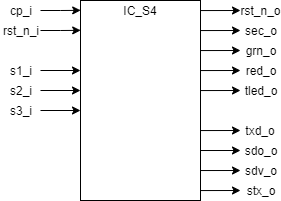
\includegraphics[scale=0.6]{../png/top.png}
	\caption{IC\_S4 Top View}
\end{figure}
\begin{figure}[h]
	\centering
	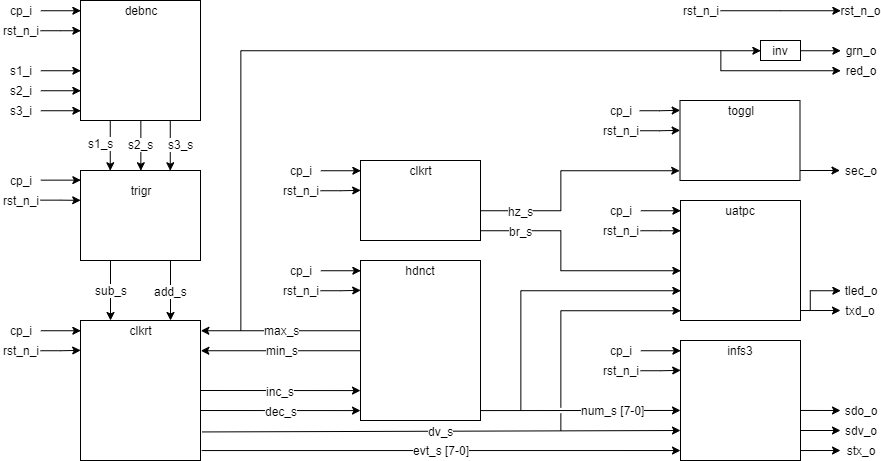
\includegraphics[scale=0.4]{../png/top-level.png}
	\caption{Top Level Block Diagram}
\end{figure}
\begin{center}
	\begin{tabular}{|l|l|c|r|}
		\hline
		\textbf{Signal} & \textbf{Pin} & \textbf{Direction} & \textbf{Description} \\
		\hline
		\hline
		rst\_n\_i & E6 & IN & Reset, active low \\
		\hline
		cp\_i & H6 & IN & Syscp, @ 12MHz \\
		\hline
		s1\_i & L12 & IN & Sensor 1 \\
		\hline
		s2\_i & J12 & IN & Sensor 2 \\
		\hline
		s3\_i & J13 & IN & Sensor 3 \\
		\hline
		rst\_n\_o & A8 & OUT & Reset state LED  \\
		\hline
		sec\_o & A9 & OUT & Pulse LED \\
		\hline
		grn\_o & A11 & OUT & Green LED, go ahead \\
		\hline
		red\_o & A10 & OUT & Red LED, stop, access denied \\
		\hline
		tled\_o & B10 & OUT & Transmission LED \\
		\hline
		txd\_o & K11 & OUT & Transmission RS-232-driver, 9k6,8N2,ASCII,to PC \\
		\hline
		sdi\_o & K12 & OUT & S3 data value \\
		\hline
		sdv\_o & J10 & OUT & S3 data valid \\
		\hline
		stx\_o & H10 & OUT & S3 transmission active \\
		\hline
	\end{tabular}
\end{center}
\begin{center}
	\begin{tabular}{ | p{2cm} | c | p{5cm} |}
		\hline
		\textbf{Internal Signal} & \textbf{Width} & \textbf{Description} \\
		\hline
		br\_s & 1 & 9600 baud rate signal \\
		\hline
		hz\_s & 1 & 1Hz signal \\
		\hline
		add\_s & 1 & trigger signal that someone entered \\
		\hline
		sub\_s & 1 & trigger signal that someone left \\
		\hline
		inc\_s & 1 & increment headcount signal \\
		\hline
		dec\_s & 1 & decrement headcount signal \\
		\hline
		min\_s & 1 & headcount reached min \\
		\hline
		max\_s & 1 & headcount reached max \\
		\hline
		num\_s & 8 & contains the headcount number \\
		\hline
		evh\_s & 8 & contains the current event (ASCII) \\
		\hline
	\end{tabular}
\end{center}

\newpage

\section*{Functionality}
When some one passes the sensors, the IC\_S4 will recognize if the person passing enters the room or leaves it. 
According to the event the headcounter gets adjusted (either increased or decreased). With a red LED is indicated that 
the maximum amount of people in the room is reached. Else a green LED indicates otherwise. \\ \\
\textbf{Assumptions}:
\begin{itemize}
	\item Everyone completes the enter/leave process compleatly.
	\item No one enters, when the room is full.
	\item No one leaves, when room is already empty.
\end{itemize}
\chapter{VHDL Design}

\section{debnc: Signal Debouncing}
This module debounces three incomming signals into unbounced pulsed signals. To do that it uses the module dbpul 
three times.
\begin{figure}[h]
	\centering	
	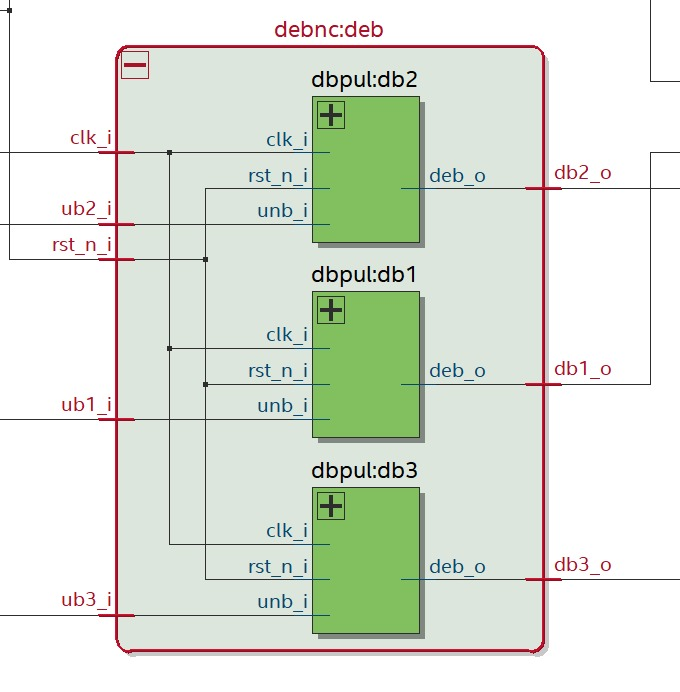
\includegraphics[scale=0.3]{../png/debnc_deb.png}
	\caption{debnc\_deb}
\end{figure}
\begin{center}
	\begin{tabular}{ | p{2cm} | c | c | p{5cm} |}
		\hline
		\textbf{Signal} & \textbf{Direction} & \textbf{Width} & \textbf{Description} \\
		\hline
	  rst\_n\_i & IN & 1 & Reset, active low \\
	  \hline
		clk\_i & IN & 1 & Syscp, @ 12MHz \\
		\hline
		ub1\_i & IN & 1 & Unbounced Input 1 \\
		\hline
		ub2\_i & IN & 1 & Unbounced Input 2 \\
		\hline
		ub3\_i & IN & 1 & Unbounced Input 3 \\
		\hline
		db1\_o & OUT & 1 & Debounced Output 1 \\
		\hline
		db2\_o & OUT & 1 & Debounced Output 2 \\
		\hline
		db3\_o & OUT & 1 & Debounced Output 3 \\
		\hline
	\end{tabular}
\end{center}

\newpage

\subsection{dbpul: Pulse Debouncer}
An unbounced signal from e.g. a Button can create multiple signals when only once pressed. To get a more reliable signal 
the input needs to be debounced. Therefor the module waits a specified amount of time when a change happens, until the 
signal is in a static state. Than this module creates a single one clock cycle pulse.
\begin{figure}[h]
	\centering	
	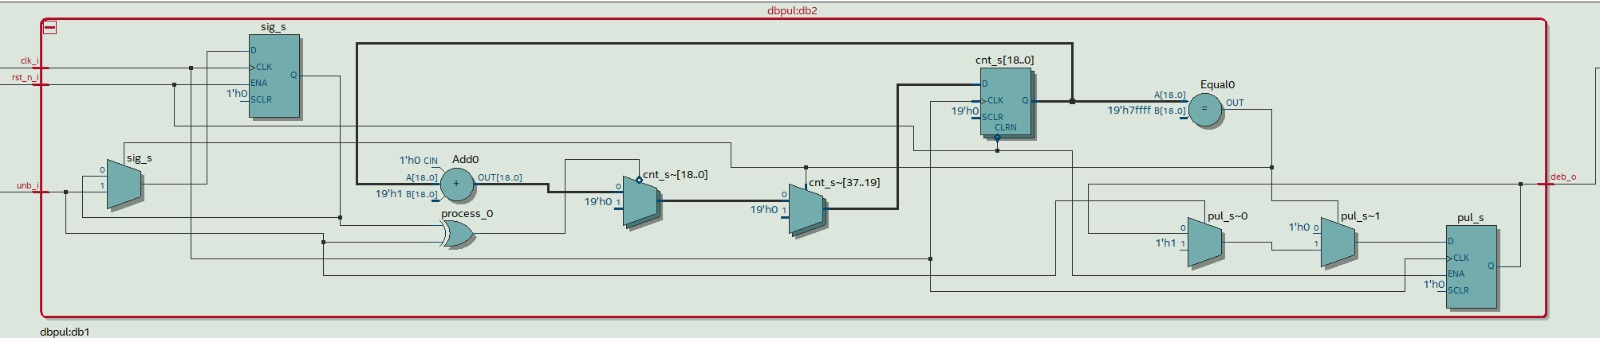
\includegraphics[scale=0.3]{../png/dbpul_db2.png}
	\caption{dbpul\_db2}
\end{figure}
\begin{center}
	\begin{tabular}{ | p{2cm} | c | c | p{5cm} |}
		\hline
		\textbf{Signal} & \textbf{Direction} & \textbf{Width} & \textbf{Description} \\
		\hline	
  	rst\_n\_i & IN & 1 &  Reset, active low \\
  	\hline
		clk\_i & IN & 1 & Syscp, @ 12MHz \\
		\hline
		unb\_i & IN & 1 & Unbounced Input \\
		\hline
		deb\_o & OUT & 1 & Debounced Output \\
		\hline
	\end{tabular}
\end{center}
\begin{center}
	\begin{tabular}{| p{2cm} | p{2cm} | p{4cm} |}
	\hline
	\textbf{Generic} & \textbf{Type} & \textbf{Description} \\
	\hline
	debounce\_width & integer & Duration of debouncing (vector size) \\
	\hline
	\end{tabular}
\end{center}

\newpage

\section{toggl: Signal Toggle}
This module works as a flipflop. Every time it gets a impulse the output toggles. It creates the hartbeat LED pulse 
from the 1Hz clock signal.
\begin{figure}[h]
	\centering	
	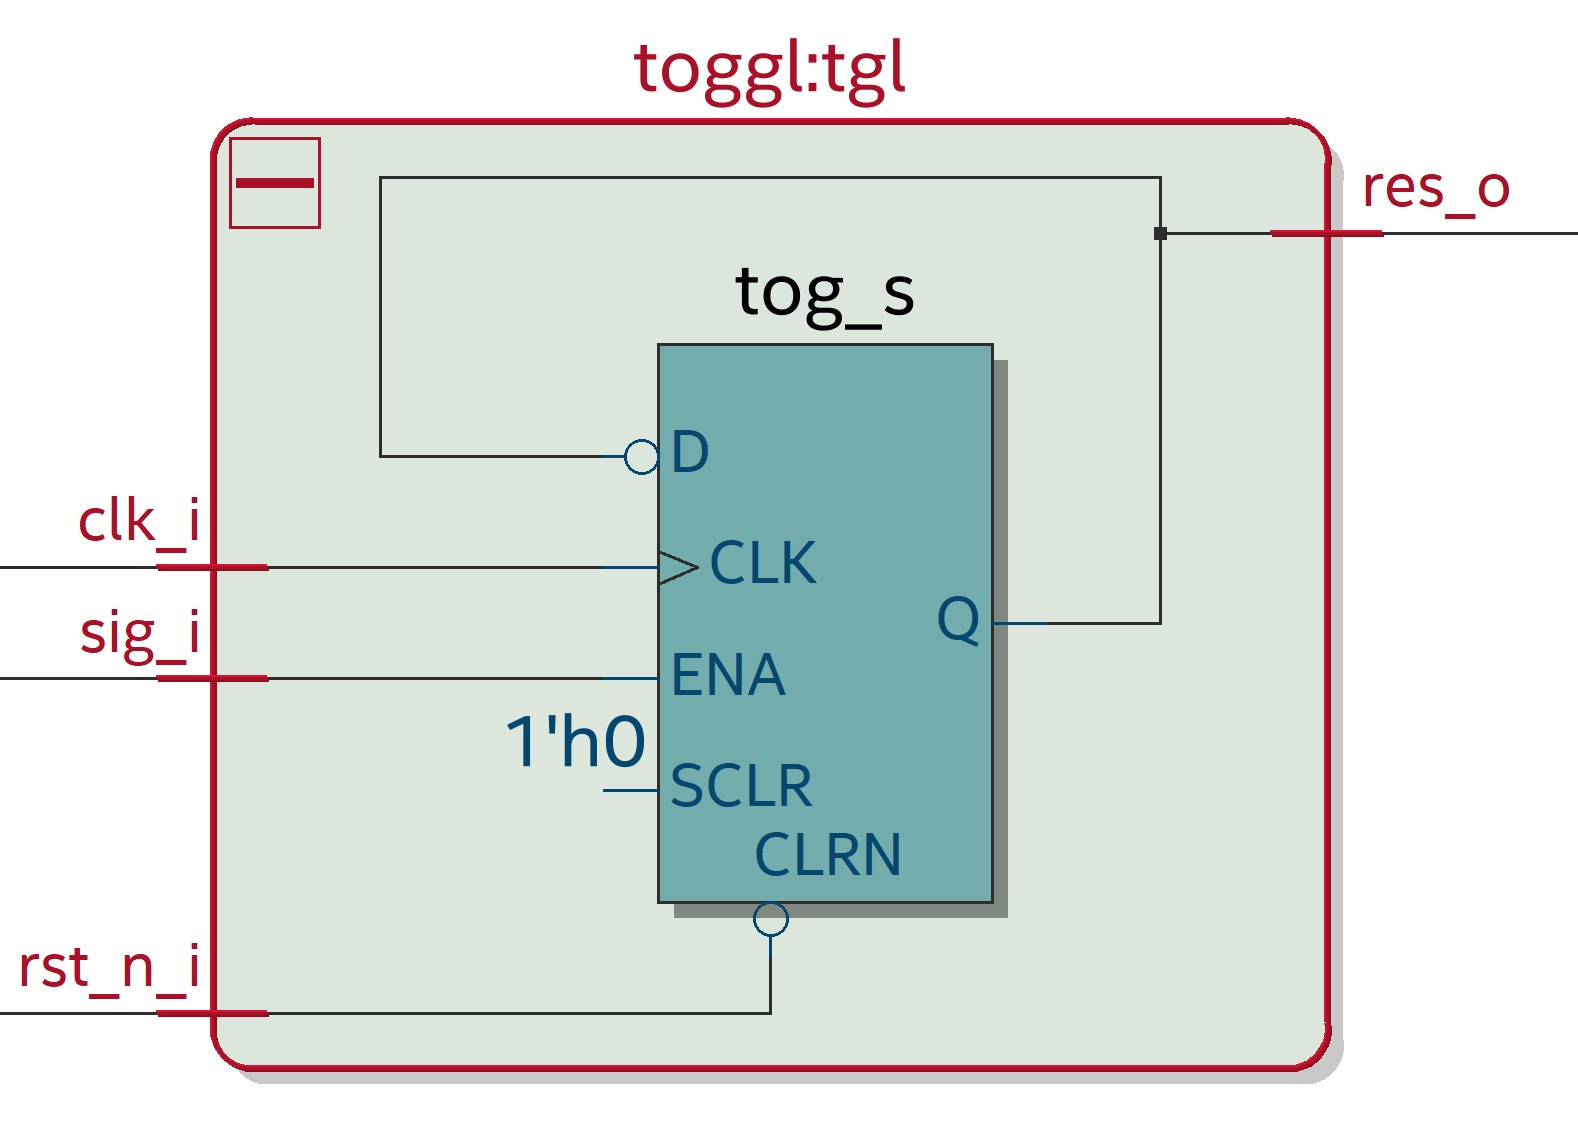
\includegraphics[scale=0.2]{../png/toggl_tgl.png}
	\caption{toggle\_tgl}
\end{figure}
\begin{center}
	\begin{tabular}{ | p{2cm} | c | c | p{5cm} |}
		\hline
		\textbf{Signal} & \textbf{Direction} & \textbf{Width} & \textbf{Description} \\
		\hline	
	  rst\_n\_i & IN & 1 & Reset, active low \\
	  \hline
		clk\_i & IN & 1 & Syscp, @ 12MHz \\
		\hline
		sig\_i & IN & 1 & Pulseing signal \\
		\hline
		res\_o & OUT & 1 & Toggeled output \\
		\hline
	\end{tabular}
\end{center}

\newpage

\section{clkrt: Clock Rate Generator}
This module generates an 1Hz signal as well as an 9600Hz baud rate. To generate those it uses the module clkgn two 
times.
\begin{figure}[h]
	\centering
	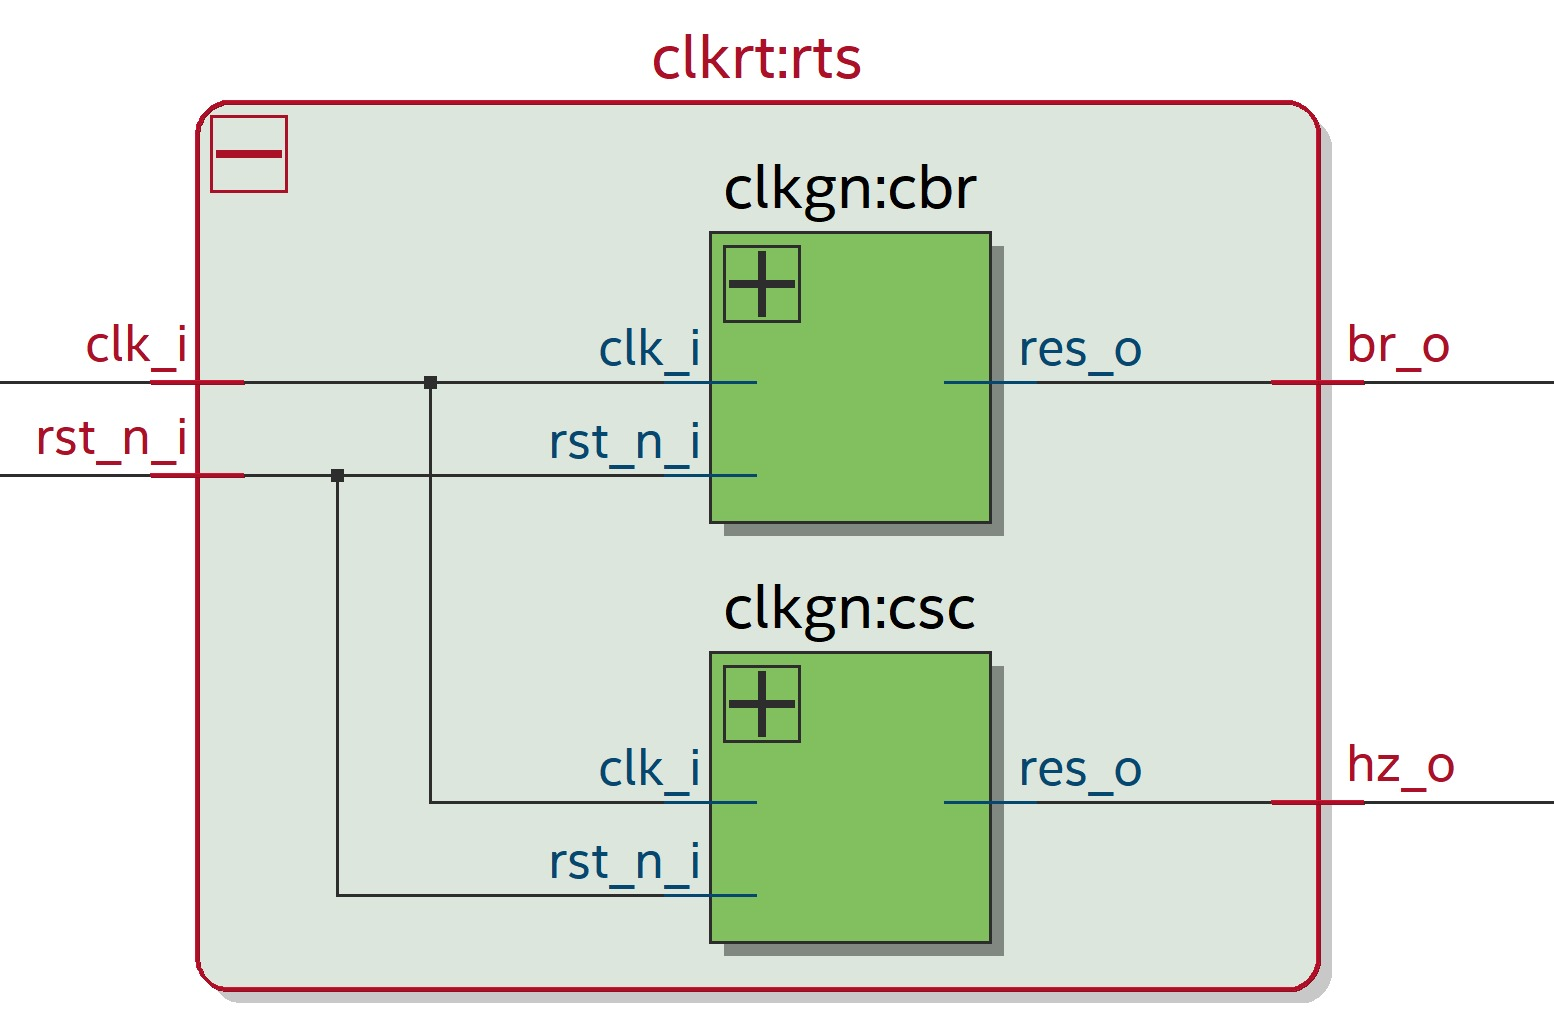
\includegraphics[scale=0.3]{../png/clkrt_rts.png}
	\caption{clkrt\_rts}
\end{figure}
\begin{center}
	\begin{tabular}{ | p{2cm} | c | c | p{5cm} |}
		\hline
		\textbf{Signal} & \textbf{Direction} & \textbf{Width} & \textbf{Description} \\
		\hline	
		rst\_n\_i & IN & 1 & Reset, active low \\
		\hline
		clk\_i & IN & 1 & Syscp, @ 12MHz \\
		\hline
		br\_o & OUT & 1 & Baud Rate @9600Hz \\
		\hline
		hz\_o & OUT & 1 & Alive Pulse @1Hz \\
		\hline
	\end{tabular}
\end{center}

\newpage

\subsection{clkgn: Clock Generator}
This module has a counter, which counts the clock cycles. When the pre-set amount of clock cycles is counted a pulsed 
is released.
\begin{figure}[h]
	\centering	
	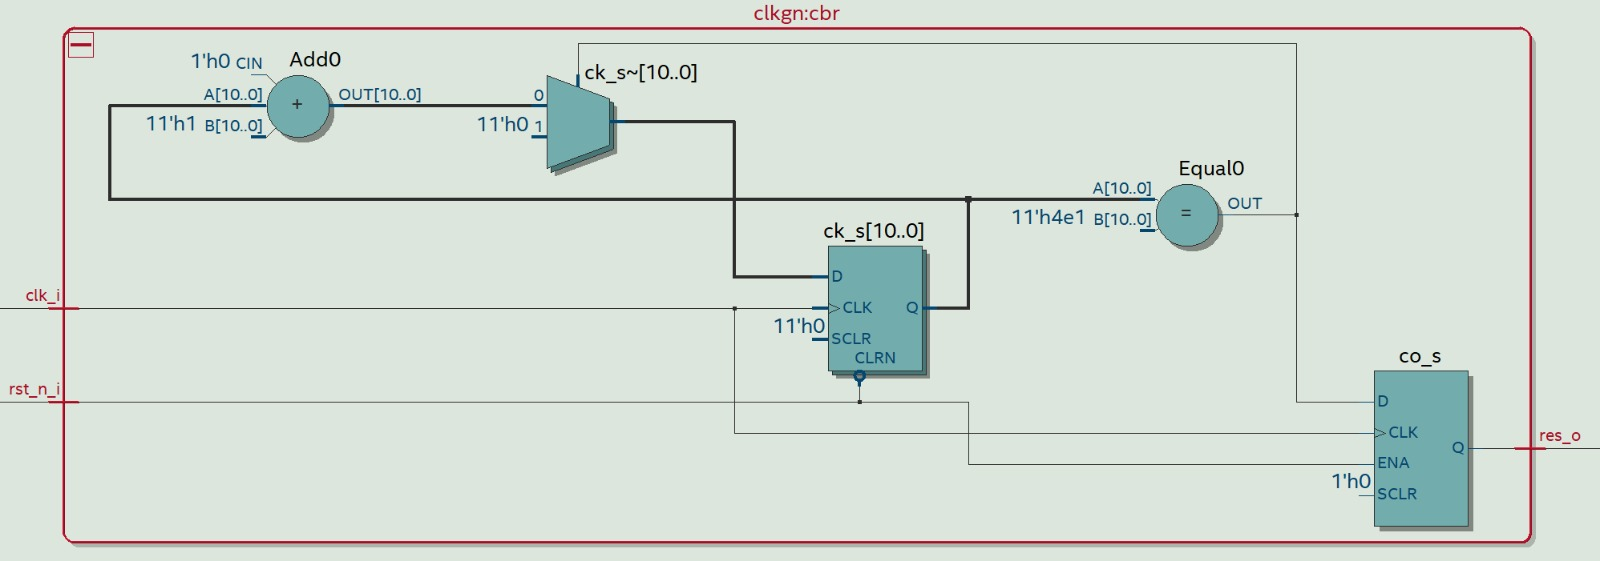
\includegraphics[scale=0.2]{../png/clkgn_cbr.png}
	\caption{clkgn\_cbr}
\end{figure}
\begin{figure}[h]
	\centering	
	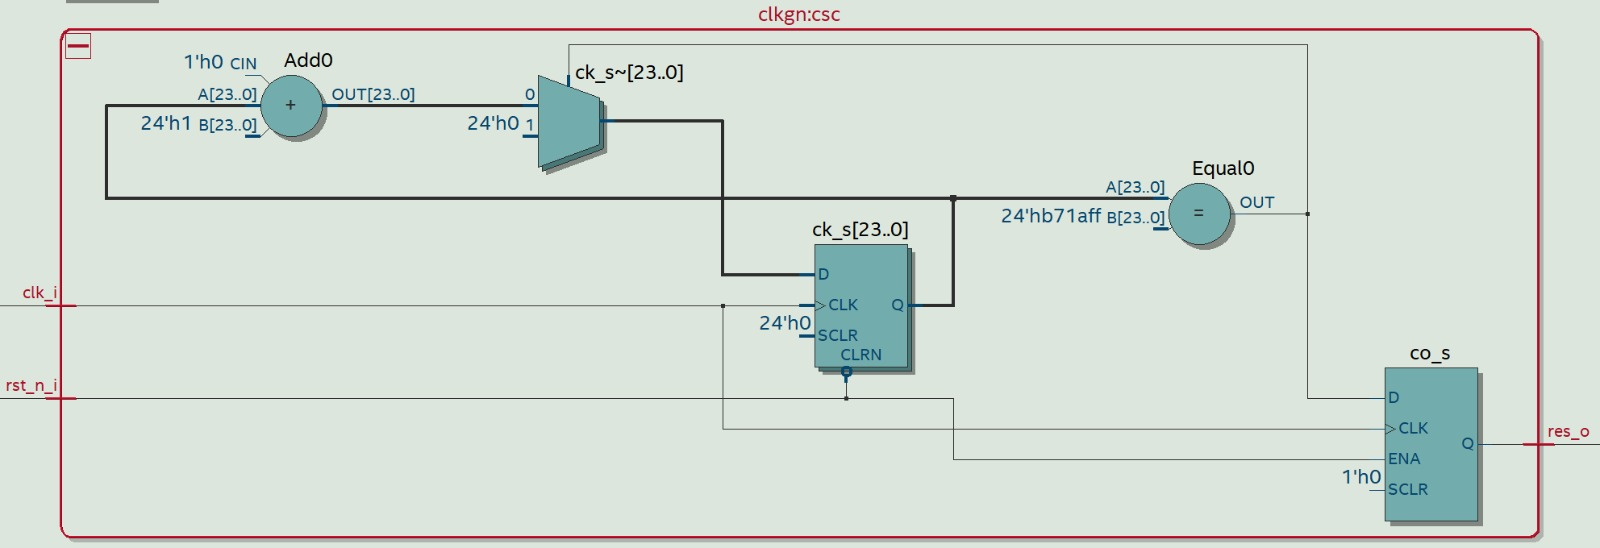
\includegraphics[scale=0.2]{../png/clkgn_csc.png}
	\caption{clkgn\_csc}
\end{figure}
\begin{center}
	\begin{tabular}{ | p{2cm} | c | c | p{5cm} |}
		\hline
		\textbf{Signal} & \textbf{Direction} & \textbf{Width} & \textbf{Description} \\
		\hline	
  	rst\_n\_i & IN & 1 & Reset, active low \\
  	\hline
		clk\_i & IN & 1 & Syscp, @ 12MHz \\
		\hline
		res\_o & OUT & 1 & Resulting Ticks \\
		\hline
	\end{tabular}
\end{center}
\begin{center}
	\begin{tabular}{| p{2cm} | p{2cm} | p{4cm} |}
	\hline
	\textbf{Generic} & \textbf{Type} & \textbf{Description} \\
	\hline
	cnt\_width & integer & Counter bit vector \\
	\hline
	div\_cnt & integer & Clock cycle durations \\	
	\hline
	\end{tabular}
\end{center}

\newpage

\section{trigr: Sensor Handling}
This module handles the debounced and pulsed sensor inputs and detects the events. It can recognize if someone is entering 
or leaving the room. According to the detection a signal is send.
\begin{figure}[h]
	\centering	
	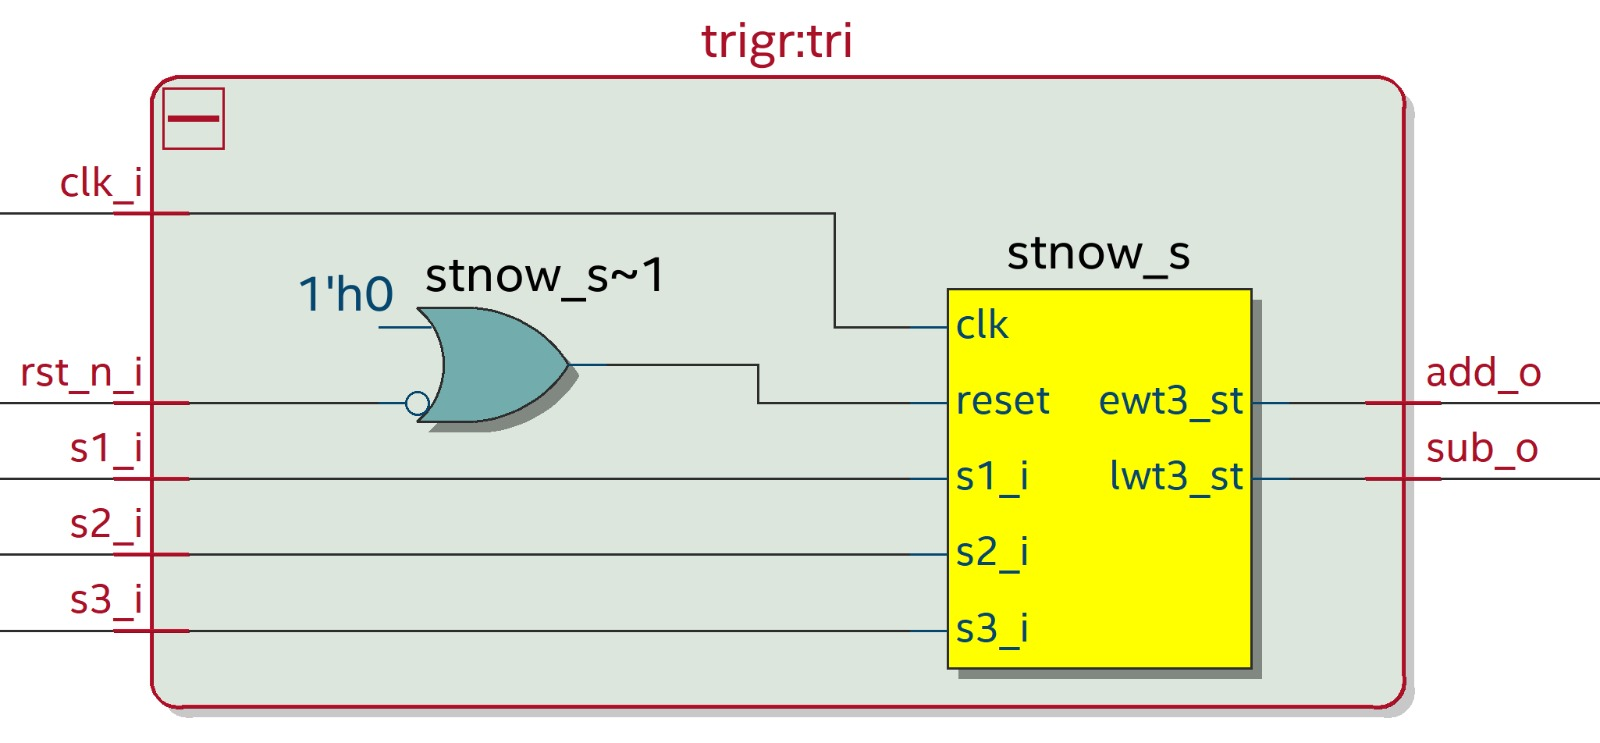
\includegraphics[scale=0.2]{../png/trigr_tri.png}
	\caption{trigr\_tri}
\end{figure}
\begin{center}
	\begin{tabular}{ | p{2cm} | c | c | p{5cm} |}
		\hline
		\textbf{Signal} & \textbf{Direction} & \textbf{Width} & \textbf{Description} \\
		\hline	
		rst\_n\_i & IN & 1 & Reset, active low \\
		\hline
		clk\_i & IN & 1 & Syscp, @ 12MHz \\
		\hline
		s1\_i & IN & 1 & Sensor 1 \\
		\hline
		s2\_i & IN & 1 & Sensor 2 \\
		\hline
		s3\_i & IN & 1 & Sensor 3 \\
		\hline
		add\_o & OUT & 1 & Person entered \\
		\hline
		sub\_o & OUT & 1 & Person left \\
		\hline
	\end{tabular}
\end{center}

\newpage

\subsection*{trigr - Finite State Machine}
\begin{figure}[h]
	\centering	
	\includegraphics[scale=0.4]{../png/trigger.png}
	\caption{Trigger FSM}
\end{figure}
\begin{center}
 \begin{tabular}{| p{4cm} | p{7cm} |}
	 \hline
	 \textbf{State Name} & \textbf{Description} \\
	 \hline
	 init\_st & wait for either sensor 1 or sensor 2 triggered \\
	 \hline
	 ewt1\_st & someone entering, sensor 1 triggered wait for sensor 2 \\
	 \hline
	 lwt1\_st & someone leaving, sensor 3 triggered wait for sensor 2 \\
	 \hline
	 ewt2\_st & someone entering, sensor 2 triggered wait for sensor 3 \\
	 \hline
	 lwt2\_st & someone leaving, sensor 2 triggered wait for sensor 1 \\
	 \hline
	 ewt3\_st & someone entering, sensor 3 triggered -> back to init \\
	 \hline
	 lwt3\_st & someone leaving, sensor 1 triggered -> back to init \\
	 \hline
 \end{tabular}
\end{center}

\newpage

\section{hdcnt: HeadCounter}
This module stores the current number of people in the room. It increments or decrements the number if needed. 
Additionally it indecates if min or max number of people is reached.
\begin{figure}[h]
	\centering	
	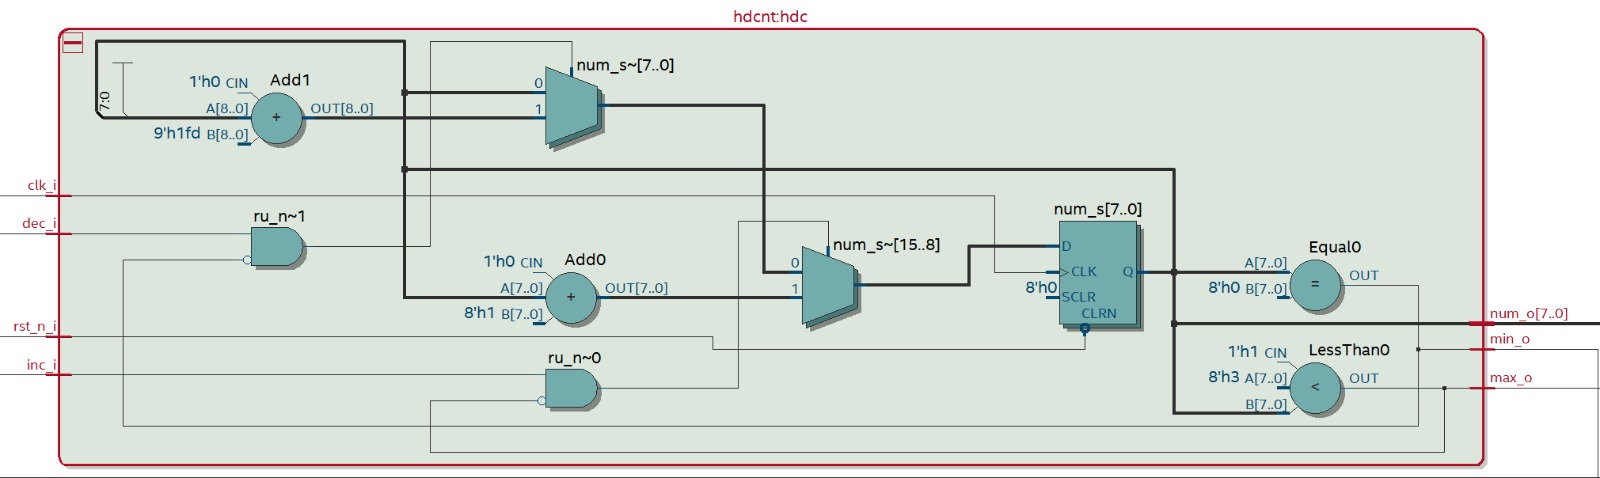
\includegraphics[scale=0.3]{../png/hdcnt_hdc.png}
	\caption{hdcnt\_hdc}
\end{figure}
\begin{center}
	\begin{tabular}{ | p{2cm} | c | c | p{5cm} |}
		\hline
		\textbf{Signal} & \textbf{Direction} & \textbf{Width} & \textbf{Description} \\
		\hline	
		rst\_n\_i & IN & 1 & Reset, active low \\
		\hline
		clk\_i & IN & 1 & Syscp, @ 12MHz \\
		\hline
		inc\_i & IN & 1 & Increment Counter Signal \\
		\hline
		dec\_i & IN & 1 & Decrement Counter Signal \\
		\hline
		min\_o & OUT & 1 & Min persons in room \\
		\hline
		max\_o & OUT & 1 & Max persons in room \\
		\hline
		num\_o & OUT & 8 & Contains the number \\
		\hline
	\end{tabular}
\end{center}
\begin{center}
	\begin{tabular}{| p{2cm} | p{2cm} | p{4cm} |}
		\hline
		\textbf{Generic} & \textbf{Type} & \textbf{Description} \\
		\hline
		cnt\_width & integer & Counter bit vector size  \\
		\hline
		max\_cnt & integer & Trigger number \\
		\hline
	\end{tabular}	
\end{center}

\newpage

\section{cntrl: Controller}
This module controls the whole system and decides what to do next according to the inputs and the current states.
\begin{figure}[h]
	\centering	
	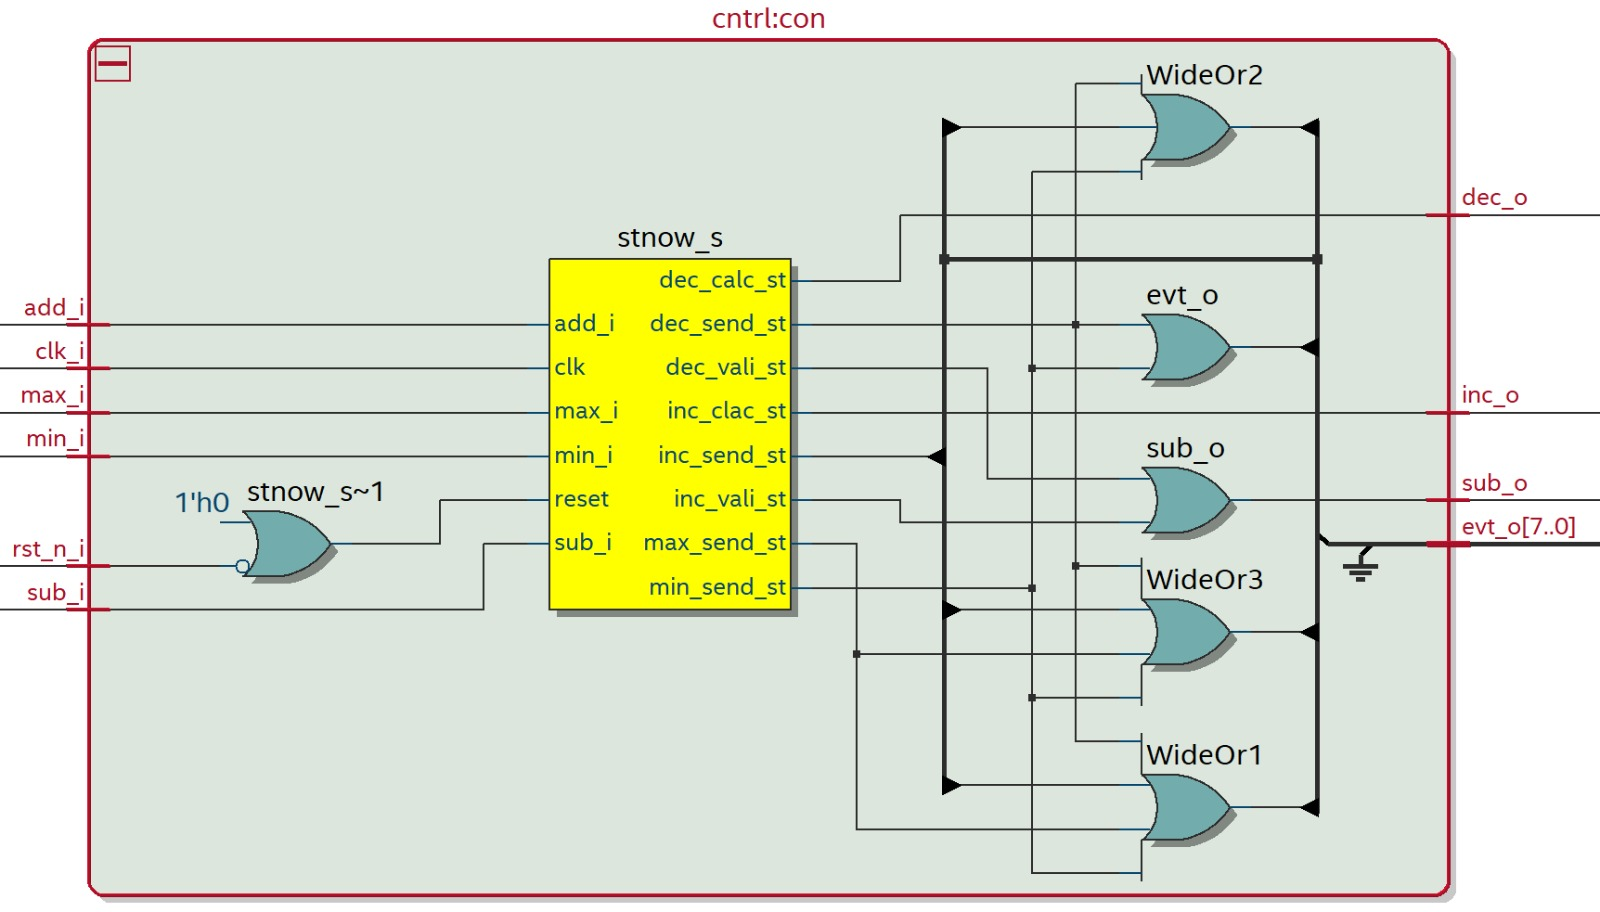
\includegraphics[scale=0.3]{../png/cntrl_con.png}
	\caption{cntrl\_con}
\end{figure}
\begin{center}
	\begin{tabular}{ | p{2cm} | c | c | p{5cm} |}
		\hline
		\textbf{Signal} & \textbf{Direction} & \textbf{Width} & \textbf{Description} \\
		\hline	
		rst\_n\_i & IN & 1 & Reset, active low \\
		\hline
		clk\_i & IN & 1 & Syscp, @ 12MHz \\
		\hline
		add\_i & IN & 1 & Person entered \\
		\hline
		sub\_i & IN & 1 & Person left \\
		\hline
		min\_i & IN & 1 & Min persons in room \\
		\hline
		max\_i & IN & 1 & Max persons in room \\
		\hline
		inc\_o & OUT & 1 & Increment Counter Signal \\
		\hline
		dec\_o & OUT & 1 & Decrement Counter Signal \\
		\hline
		evt\_o & OUT & 8 & Happened event char \\
		\hline
		sub\_o & OUT & 1 & Submitt/Send Data \\
		\hline
	\end{tabular}
\end{center}

\newpage

\subsection*{cntrl - Finite State Machine}
\begin{figure}[h]
	\centering	
	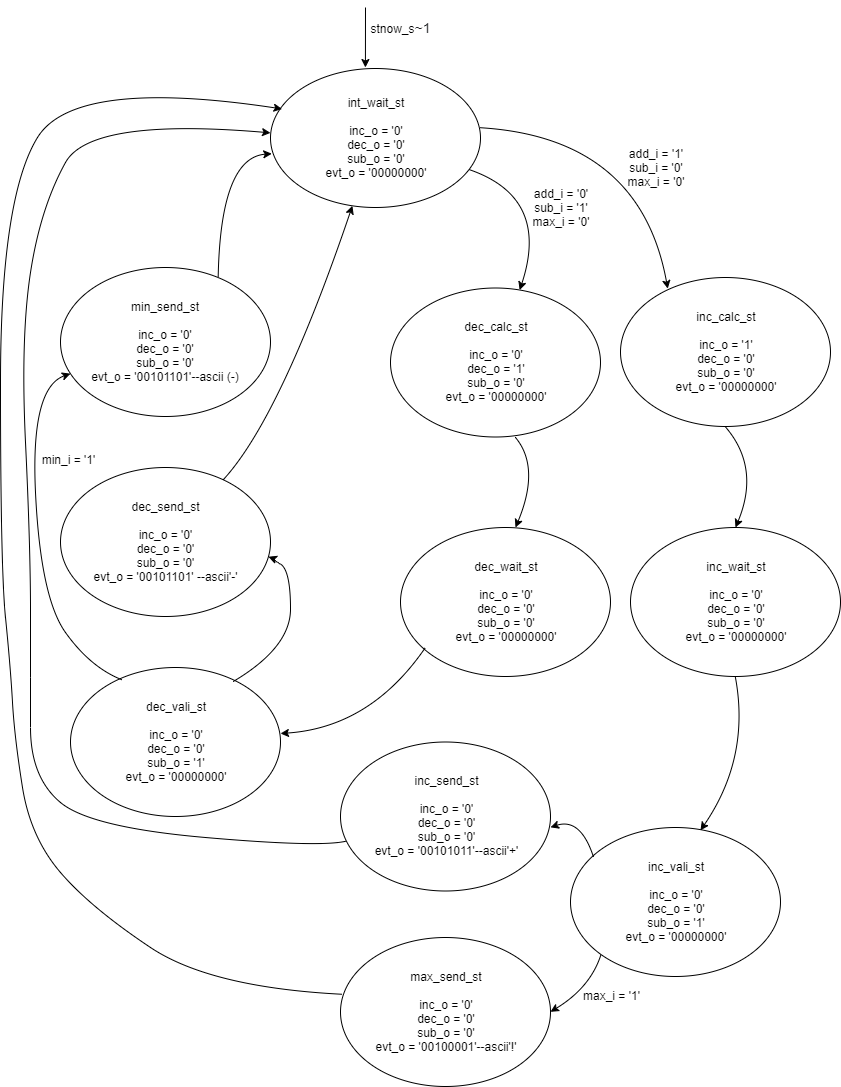
\includegraphics[scale=0.3]{../png/Control.png}
	\caption{Control FSM}
\end{figure}
\begin{center}
 \begin{tabular}{| p{4cm} | p{7cm} |}
	 \hline
	 \textbf{State Name} & \textbf{Description} \\
	 \hline
	 ini\_wait\_st & wait until \\
	 \hline
	 inc\_clac\_st & send increase signal to headcounter \\
	 \hline
	 dec\_calc\_st & send decrease signal to headcounter \\
	 \hline
	 inc\_wait\_st & wait until headcount calculated \\
	 \hline
	 dec\_wait\_st & wait until headcount calculated \\
	 \hline
	 inc\_vali\_st & done calculating, check if max \\
	 \hline
	 dec\_vali\_st & done calculating, check if min \\
	 \hline
	 inc\_send\_st & start sending num and ascii \\
	 \hline
	 dec\_send\_st & start sending num and ascii \\
	 \hline
	 min\_send\_st & start sending num and ascii \\
	 \hline
	 max\_send\_st & start sending num and ascii \\
	 \hline
 \end{tabular}
\end{center}

\newpage

\section{uatpc: UART to PC}
This module connects the IC\_S4 to a PC via the RS232. It uses a 9600 baud rate, 8 bit, no parity and 1 stop bit. When 
the send/data valid bit is received it starts to send the number bit by bit.
\begin{figure}[h]
	\centering	
	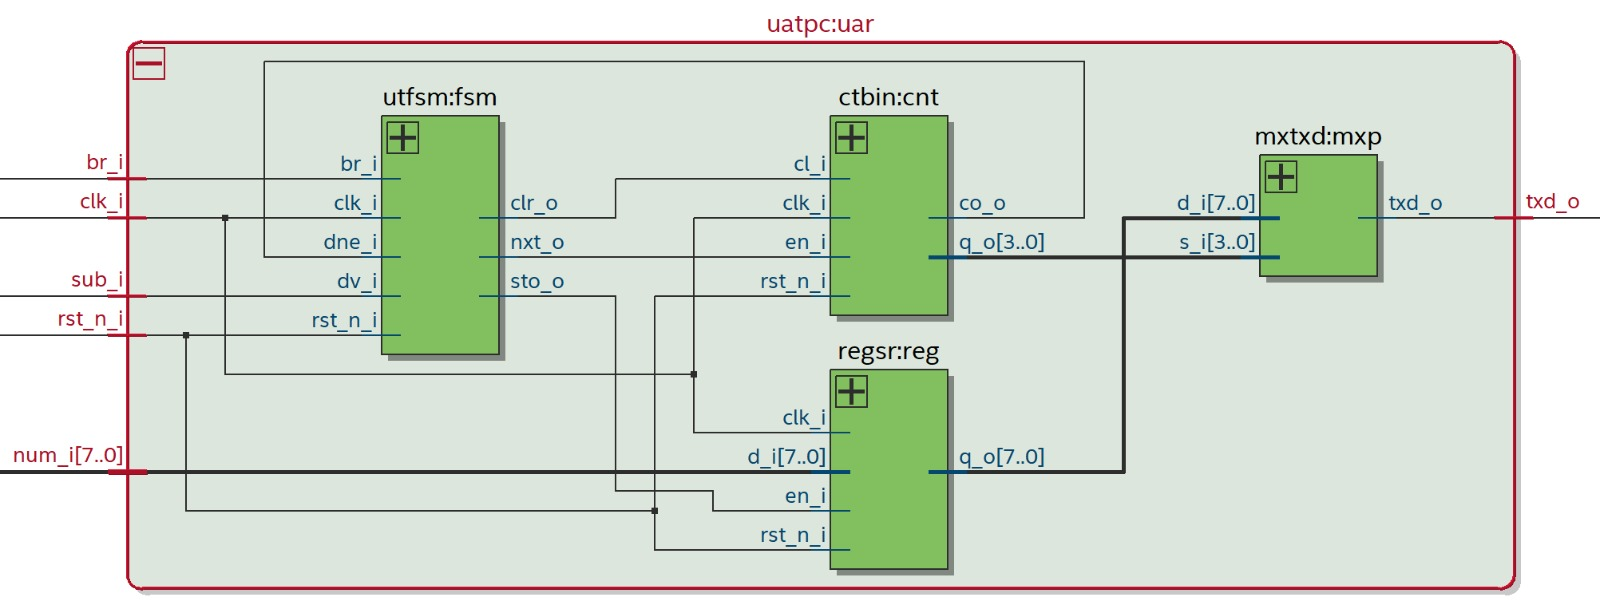
\includegraphics[scale=0.3]{../png/uatpc_uar.png}
	\caption{uatpc\_uar}
\end{figure}
\begin{center}
	\begin{tabular}{ | p{2cm} | c | c | p{5cm} |}
		\hline
		\textbf{Signal} & \textbf{Direction} & \textbf{Width} & \textbf{Description} \\
		\hline	
  	rst\_n\_i & IN & 1 & Reset, active low\\
  	\hline
		clk\_i & IN & 1 & Syscp, @ 12MHz \\
		\hline
		br\_i & IN & 1 & Baud rate \\
		\hline
		sub\_i & IN & 1 & Submitt/Send Data \\
		\hline
		num\_i & IN & 8 & Headcount number \\
		\hline
		txd\_o & OUT & 1 & Serial output \\
		\hline
	\end{tabular}
\end{center}

\newpage

\subsection{regsr: Register to store bits}
To secure the number it gets loaded and stored in the register until something new is stored.
\begin{figure}[h]
	\centering	
	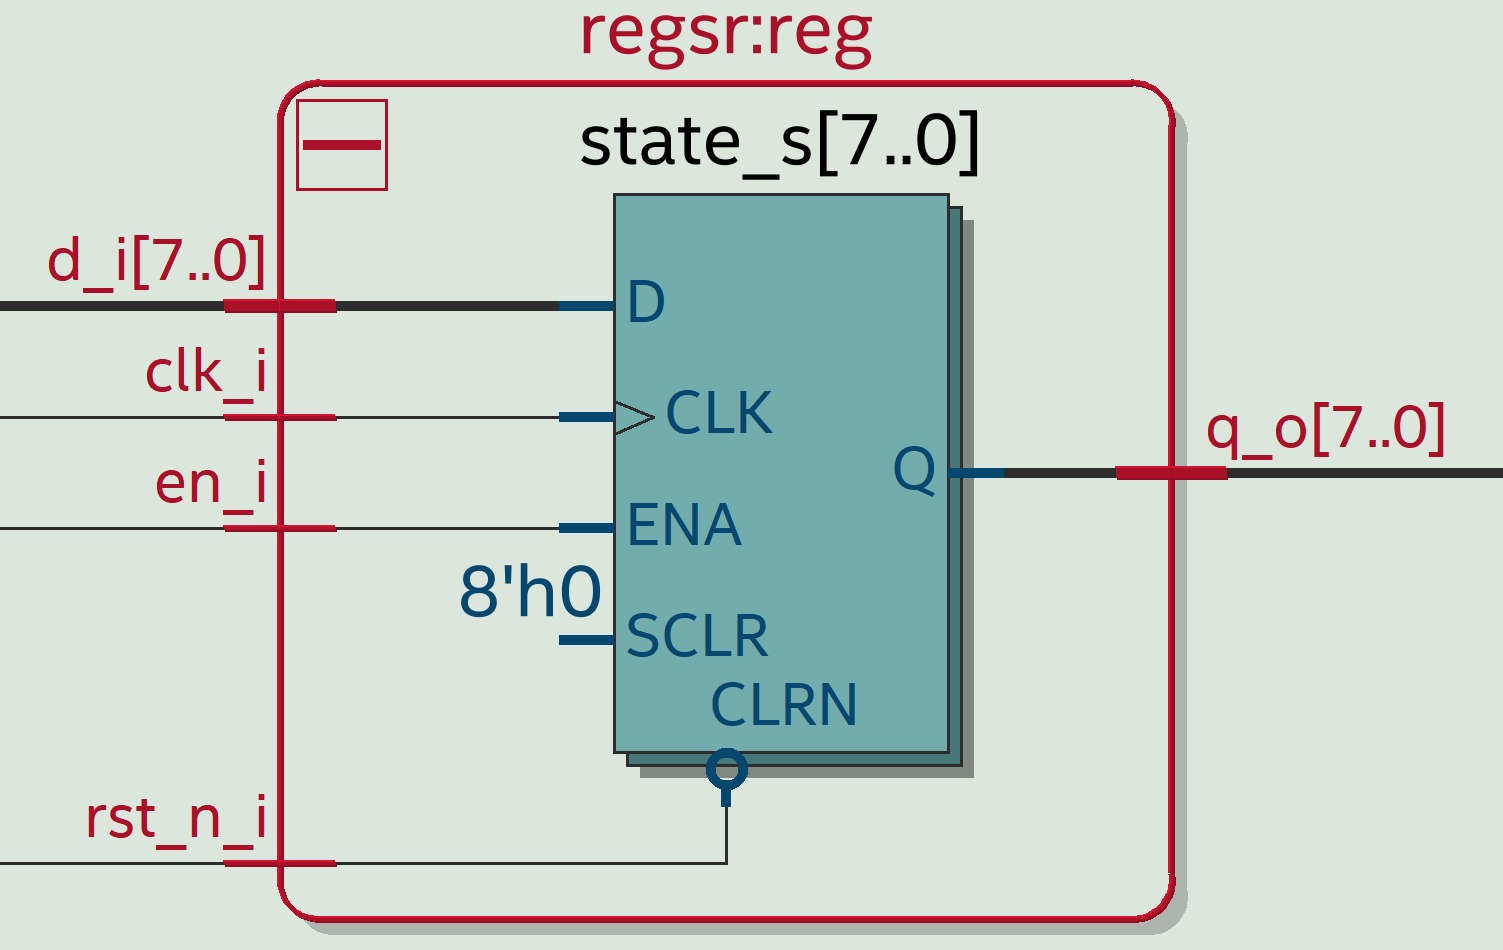
\includegraphics[scale=0.1]{../png/regsr_reg.png}
	\caption{regsr\_reg}
\end{figure}
\begin{center}
	\begin{tabular}{ | p{2cm} | c | c | p{5cm} |}
		\hline
		\textbf{Signal} & \textbf{Direction} & \textbf{Width} & \textbf{Description} \\
		\hline	
 		rst\_n\_i & IN & 1 & Reset, active low \\
 		\hline
		clk\_i & IN & 1 & Syscp, @ 12MHz \\
		\hline
		en\_i & IN & 1 & Store Data \\
		\hline
		d\_i & IN & 1 & Input Data \\
		\hline
		q\_o & OUT & 1 & Stored Data \\
		\hline
	\end{tabular}
\end{center}
\begin{center}
	\begin{tabular}{| p{2cm} | p{2cm} | p{4cm} |}
	\hline
	\textbf{Generic} & \textbf{Type} & \textbf{Description} \\
	\hline
	dta\_width & integer & Data bit vector size \\
	\hline
	\end{tabular}
\end{center}

\newpage

\subsection{ctbin: Binary Counter}
This binary counter counts until a pre-set value. It increments, when an enable counter signal is received. The current 
number and the carry can always be seen.
\begin{figure}[h]
	\centering	
	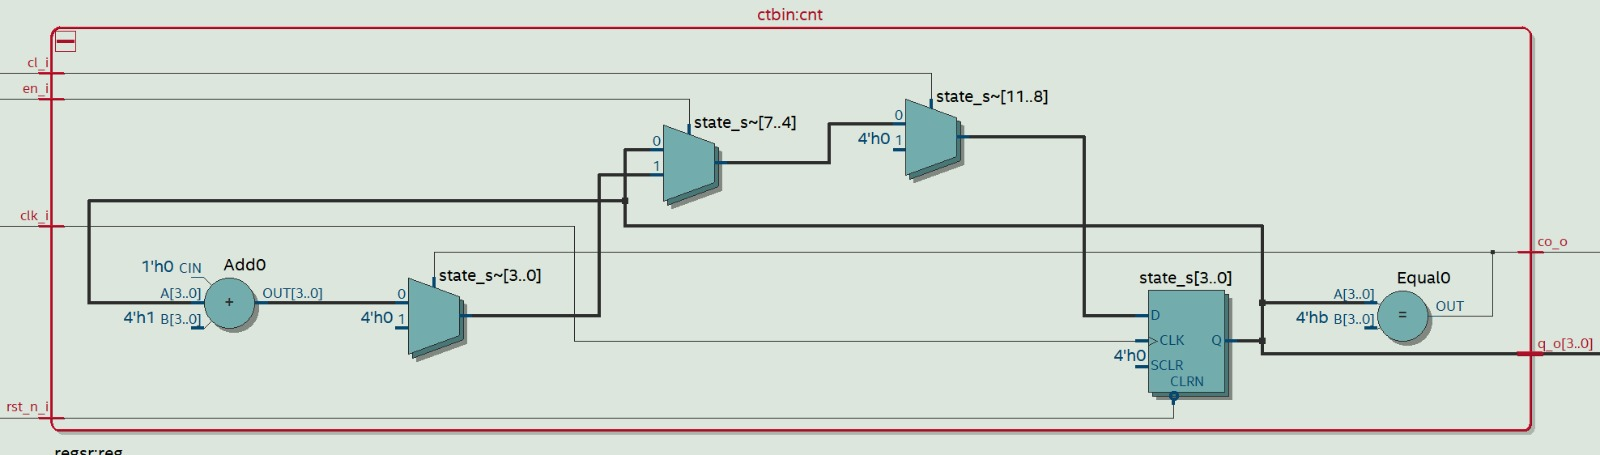
\includegraphics[scale=0.2]{../png/ctbin_cnt.png}
	\caption{ctbin\_cnt}
\end{figure}
\begin{center}
	\begin{tabular}{ | p{2cm} | c | c | p{5cm} |}
		\hline
		\textbf{Signal} & \textbf{Direction} & \textbf{Width} & \textbf{Description} \\
		\hline	
 		 rst\_n\_i & IN & 1 & Reset, active low \\
 		 \hline
		clk\_i & IN & 1 & Syscp, @ 12MHz \\
		\hline
		en\_i & IN & 1 & Enable Count \\
		\hline
		cl\_i & IN & 1 & Clear Counter \\
		\hline
		co\_o & OUT & 1 & Carry Out \\
		\hline
		q\_o & OUT & 4 & Counter Value \\
		\hline
	\end{tabular}
\end{center}
\begin{center}
	\begin{tabular}{| p{2cm} | p{2cm} | p{4cm} |}
		\hline
		\textbf{Generic} & \textbf{Type} & \textbf{Description} \\
		\hline
 		cnt\_width & integer & Counter bit vector size \\
		\hline
		cnt\_max & integer & Trigger number \\
		\hline
	\end{tabular}	
\end{center}

\newpage

\subsection{mxtxd: Multiplexer for TXD}
This multiplexer has some special states, where it has the required stopbit and initial state, for the UART transmission 
build in. In total it pushes 10 bits one by one.
\begin{figure}[h]
	\centering	
	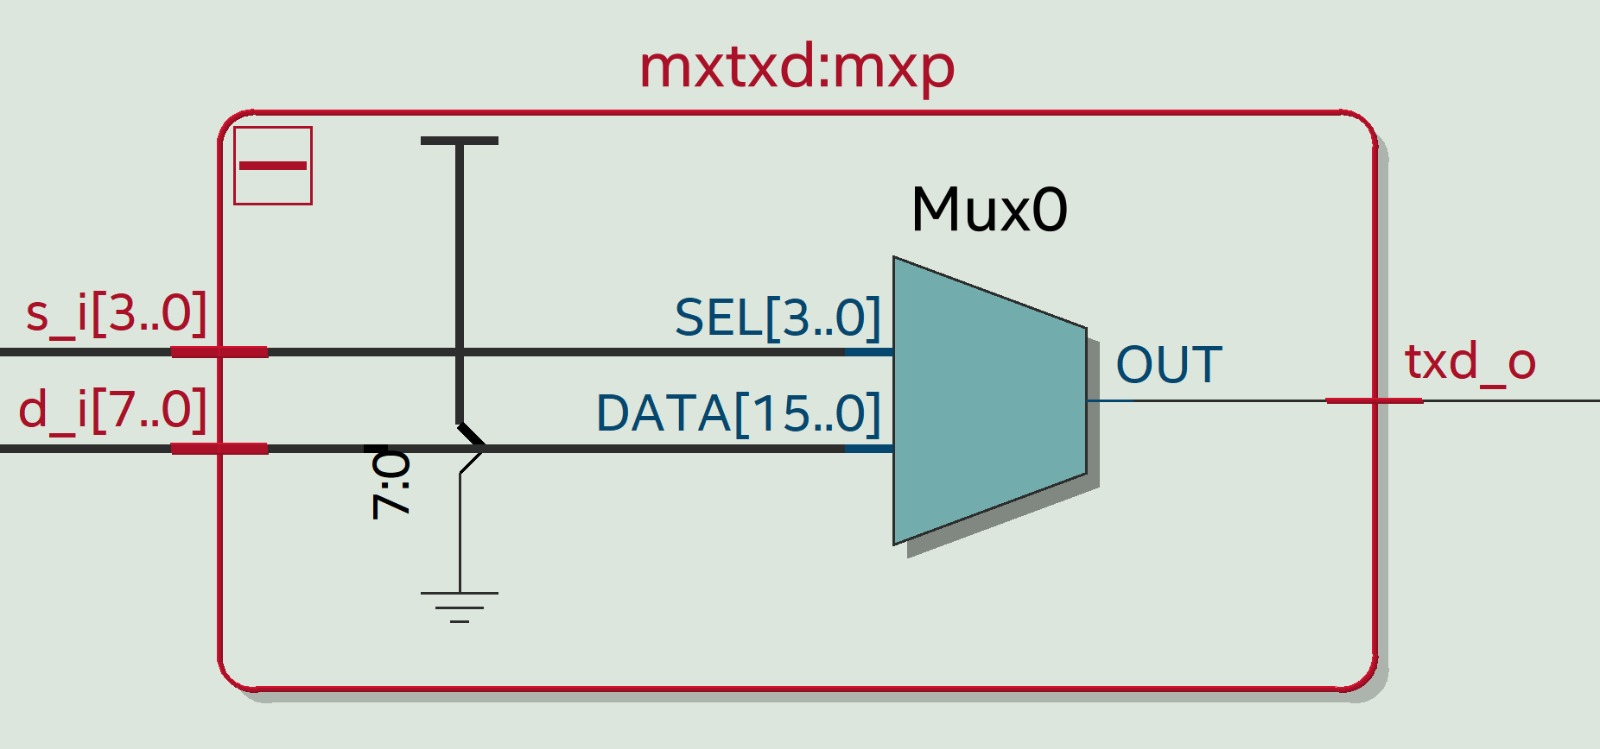
\includegraphics[scale=0.2]{../png/mxtxd_mxp.png}
	\caption{mxtxd\_mxp}
\end{figure}
\begin{center}
	\begin{tabular}{ | p{2cm} | c | c | p{5cm} |}
		\hline
		\textbf{Signal} & \textbf{Direction} & \textbf{Width} & \textbf{Description} \\
		\hline
		s\_i & IN & 4 & Bit position \\
		\hline
		d\_i & IN & 8 & Bit vector \\
		\hline
		txd\_o & OUT & 1 & Txd, Serial Output \\
		\hline
	\end{tabular}
\end{center} 

\newpage

\subsection{utfsm: FSM for UART}
This module contains the FSM for the UART.
\begin{figure}[h]
	\centering	
	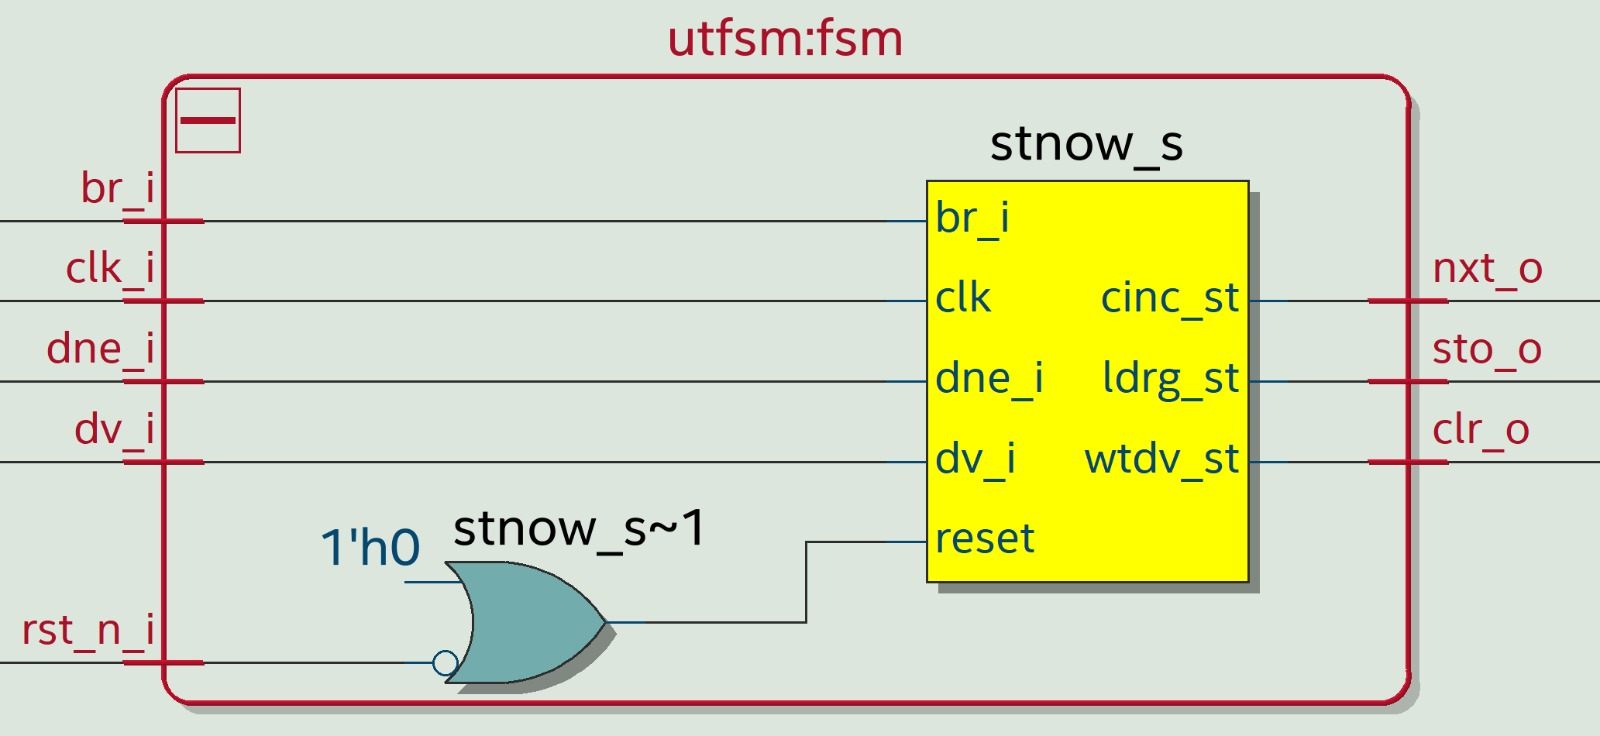
\includegraphics[scale=0.2]{../png/utfsm_fsm.png}
	\caption{utfsm\_fsm}
\end{figure}
\begin{center}
	\begin{tabular}{ | p{2cm} | c | c | p{5cm} |}
		\hline
		\textbf{Signal} & \textbf{Direction} & \textbf{Width} & \textbf{Description} \\
		\hline	
		rst\_n\_i & IN & 1 & Reset, active low \\
		\hline
		clk\_i & IN & 1 & Syscp, @ 12MHz \\
		\hline
		dv\_i  & IN & 1 & Have new RTC or GPS-Data \\
		\hline
		br\_i  & IN & 1 & Baud-Rate to ena Counter \\
		\hline
		dne\_i & IN & 1 & Last Bit transmitted \\
		\hline
		sto\_o & OUT & 1 & enable register load \\
		\hline
		clr\_o & OUT & 1 & clear Bit-Counters \\
		\hline
		nxt\_o & OUT & 1 & next Bit, inc count \\
		\hline
	\end{tabular}
\end{center}

\newpage

\subsection*{utfsm - Finite State Machine}
\begin{figure}[h]
	\centering	
	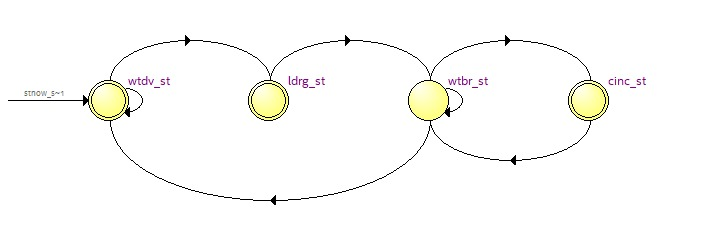
\includegraphics[scale=0.5]{../png/Uart.png}
	\caption{Uart FSM}
\end{figure}
\begin{center}
 \begin{tabular}{| p{4cm} | p{7cm} |}
	 \hline
	 \textbf{State Name} & \textbf{Description} \\
	 \hline
	 wtdv\_st & wait until data valid \\
	 \hline
	 ldrg\_st & load data in register \\
	 \hline
	 wtbr\_st & wait till baud rate is 1 or goto wtdv when done transmitting \\
	 \hline
	 cinc\_st & get next bit (increment counter) \\
	 \hline
 \end{tabular}
\end{center}

\newpage

\section{infs3: Interface to S3}
This module connects the IC\_S4 to a IC\_S3 via a 3-wire-interface. It passes the current event as well as the number 
of people in the room.
\begin{figure}[h]
	\centering	
	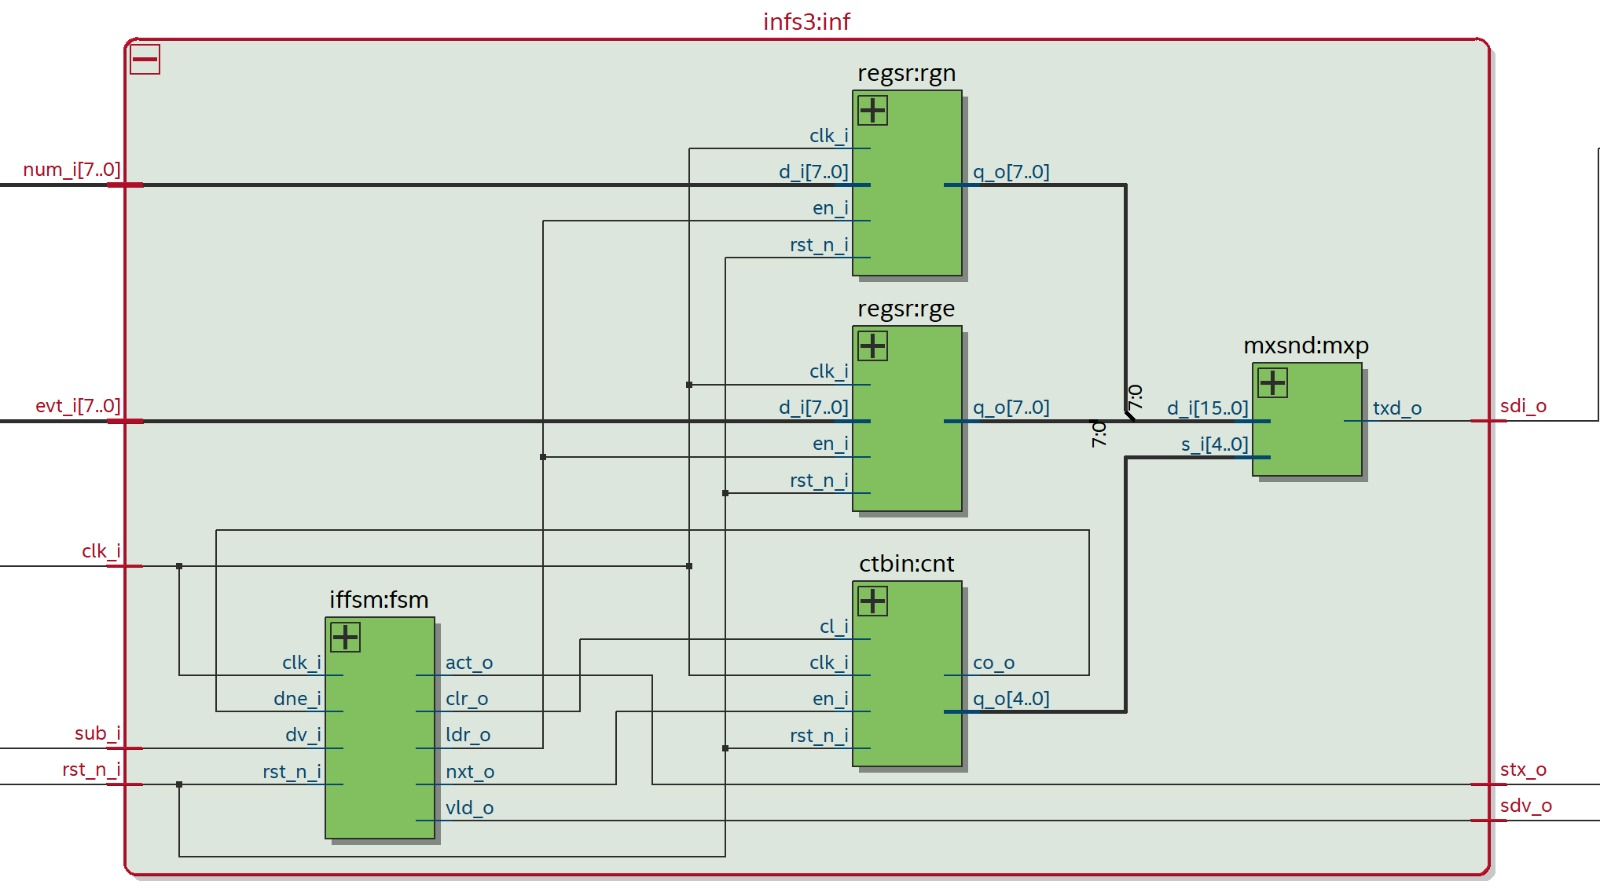
\includegraphics[scale=0.3]{../png/infs3_inf.png}
	\caption{infs3\_inf}
\end{figure}
\begin{center}
	\begin{tabular}{ | p{2cm} | c | c | p{5cm} |}
		\hline
		\textbf{Signal} & \textbf{Direction} & \textbf{Width} & \textbf{Description} \\
		\hline	
  	rst\_n\_i & IN & 1 & Reset, active low \\
  	\hline
		clk\_i & IN & 1 & Syscp, @ 12MHz \\
		\hline
		sub\_i & IN & 1 & Submitt/Send Data \\
		\hline
		evt\_i & IN & 8 &  Occured event char \\
		\hline
		num\_i & IN & 8 & Head count number \\
		\hline
		sdi\_o & OUT & 1 & S3 data value \\
		\hline
		sdv\_o & OUT & 1 & S3 data valid \\
		\hline
		stx\_o & OUT & 1 & S3 transmission active\\
		\hline
	\end{tabular}
\end{center}

\newpage

\subsection{regsr: Register to store bits}
To secure the number and the event they get loaded and stored in a register until something new is stored.
\begin{figure}[h]
	\centering	
	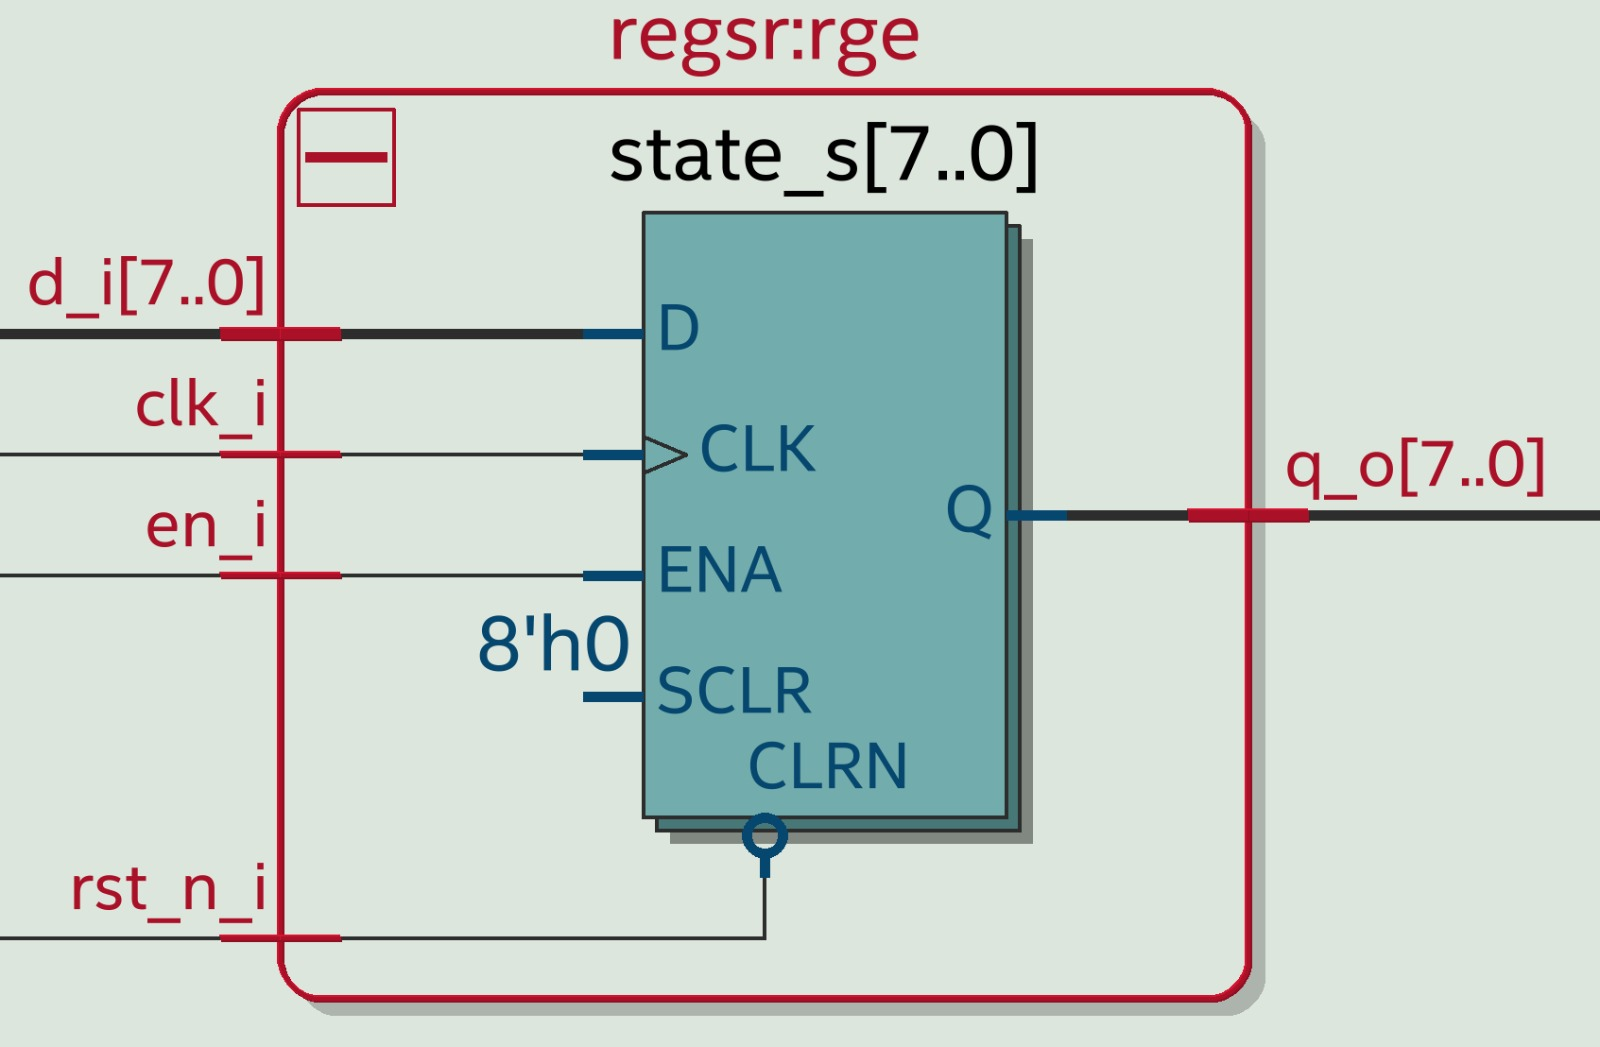
\includegraphics[scale=0.15]{../png/regsr_rge.png}
	\caption{regsr\_rge}
\end{figure}
\begin{figure}[h]
	\centering	
	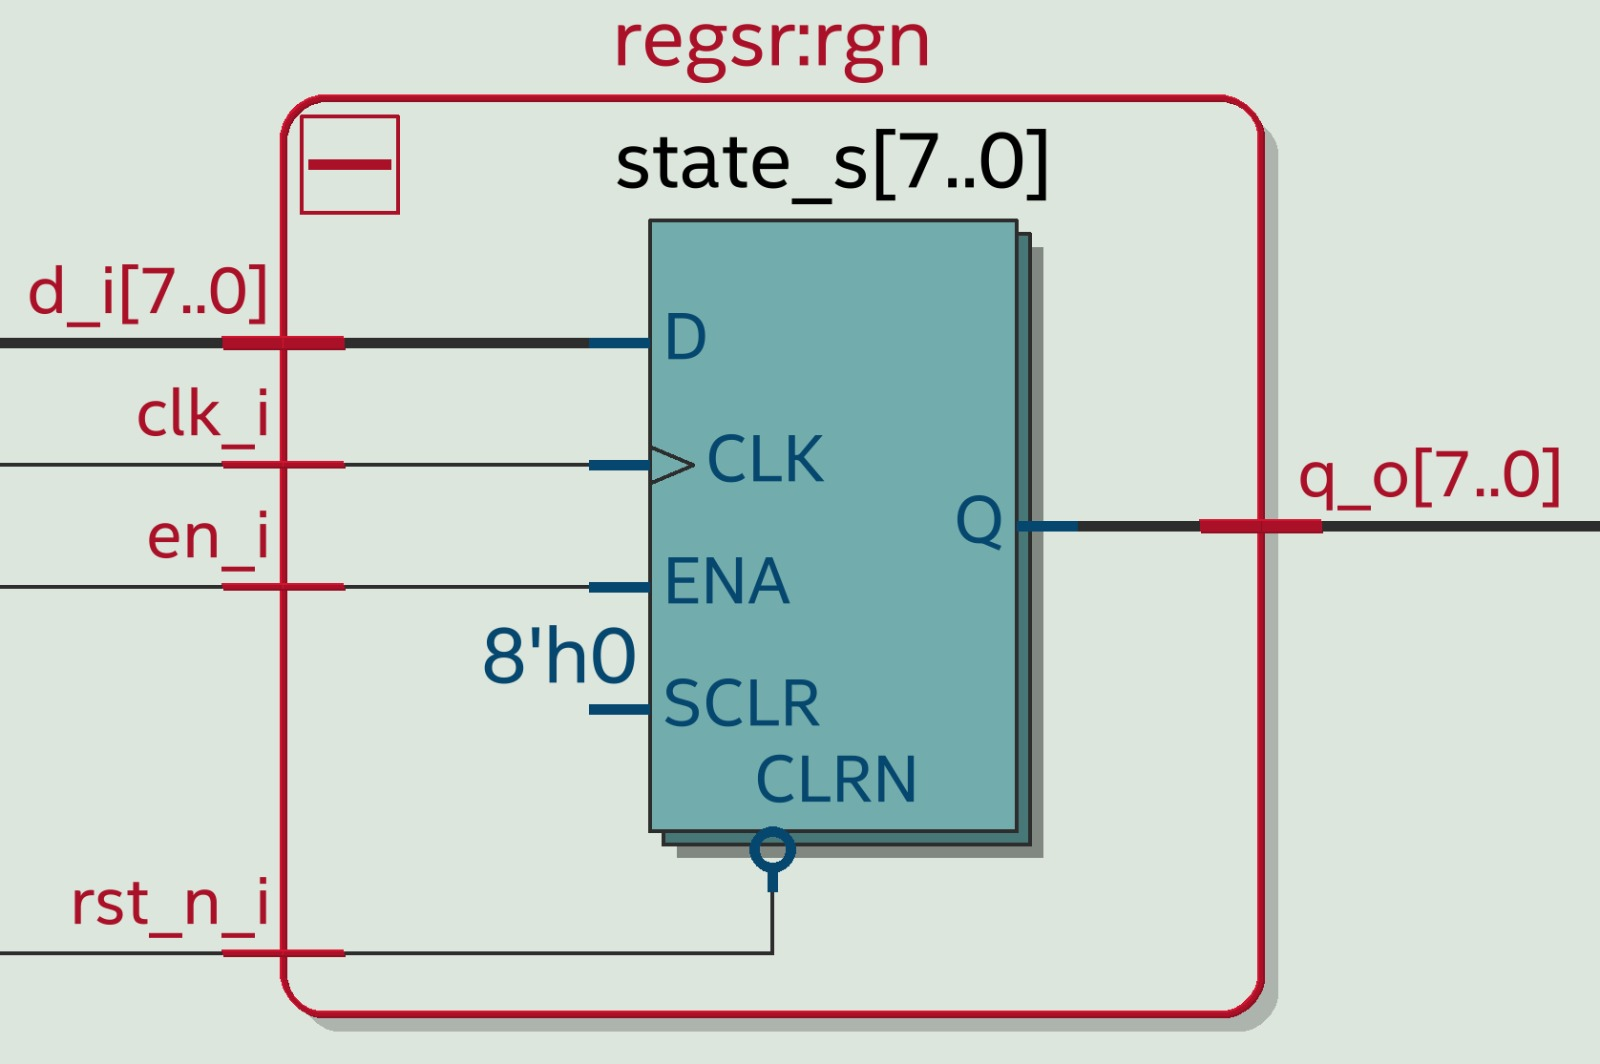
\includegraphics[scale=0.15]{../png/regsr_rgn.png}
	\caption{regsr\_rgn}
\end{figure}
\begin{center}
	\begin{tabular}{ | p{2cm} | c | c | p{5cm} |}
		\hline
		\textbf{Signal} & \textbf{Direction} & \textbf{Width} & \textbf{Description} \\
		\hline	
 		rst\_n\_i & IN & 1 & Reset, active low \\
 		\hline
		clk\_i & IN & 1 & Syscp, @ 12MHz \\
		\hline
		en\_i & IN & 1 & Store Data \\
		\hline
		d\_i & IN & 8 & Input Data \\
		\hline
		q\_o & OUT & 8 & Stored Data \\
		\hline
	\end{tabular}
\end{center}
\begin{center}
	\begin{tabular}{| p{2cm} | p{2cm} | p{4cm} |}
	\hline
	\textbf{Generic} & \textbf{Type} & \textbf{Description} \\
	\hline
	dta\_width & integer & Data bit vector size \\
	\hline
	\end{tabular}
\end{center}

\newpage

\subsection{ctbin: Binary Counter}
This binary counter counts until a pre-set value. It increments, when an enable counter signal is received. The current 
number and the carry can always be seen.
\begin{figure}[h]
	\centering	
	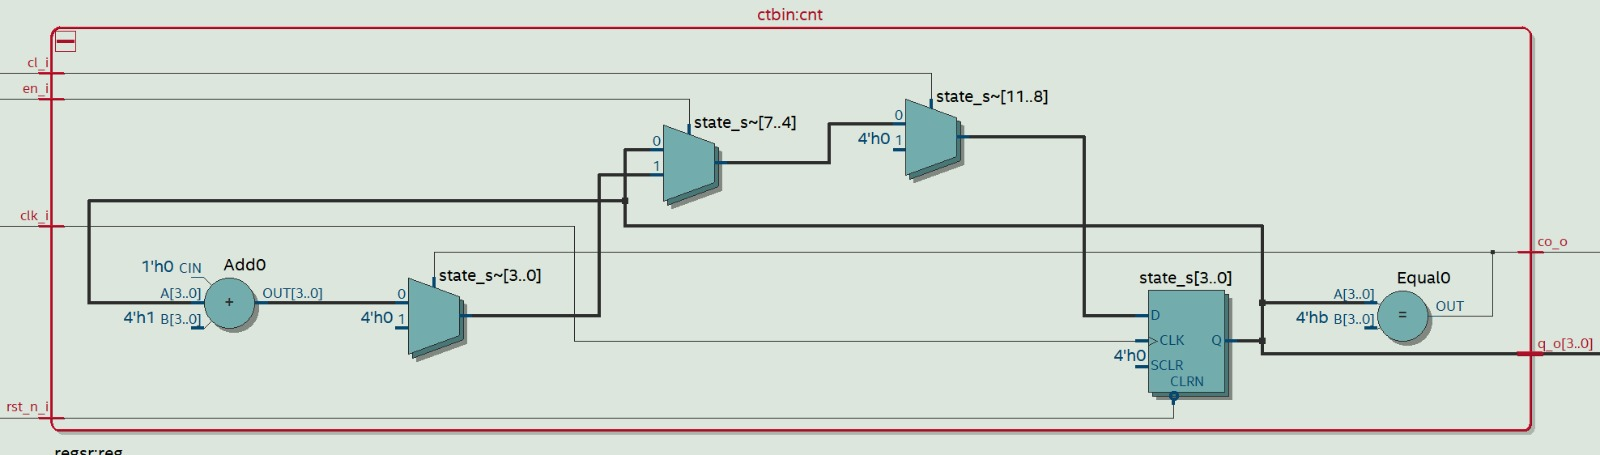
\includegraphics[scale=0.2]{../png/ctbin_cnt.png}
	\caption{ctbin\_cnt}
\end{figure}
\begin{center}
	\begin{tabular}{ | p{2cm} | c | c | p{5cm} |}
		\hline
		\textbf{Signal} & \textbf{Direction} & \textbf{Width} & \textbf{Description} \\
		\hline	
 		 rst\_n\_i & IN & 1 & Reset, active low \\
 		 \hline
		clk\_i & IN & 1 & Syscp, @ 12MHz \\
		\hline
		en\_i & IN & 1 & Enable Count \\
		\hline
		cl\_i & IN & 1 & Clear Counter \\
		\hline
		co\_o & OUT & 1 & Carry Out \\
		\hline
		q\_o & OUT & 5 & Counter Value \\
		\hline
	\end{tabular}
\end{center}
\begin{center}
	\begin{tabular}{| p{2cm} | p{2cm} | p{4cm} |}
		\hline
		\textbf{Generic} & \textbf{Type} & \textbf{Description} \\
		\hline
 		cnt\_width & integer & Counter bit vector size \\
		\hline
		cnt\_max & integer & Trigger number \\
		\hline
	\end{tabular}	
\end{center}

\newpage

\subsection{mxsnd: Multiplexer for Interface to S3}
This multiplexer has in total 17 bits to push one by one. One of them is a initial 0 bit.
\begin{figure}[h]
	\centering	
	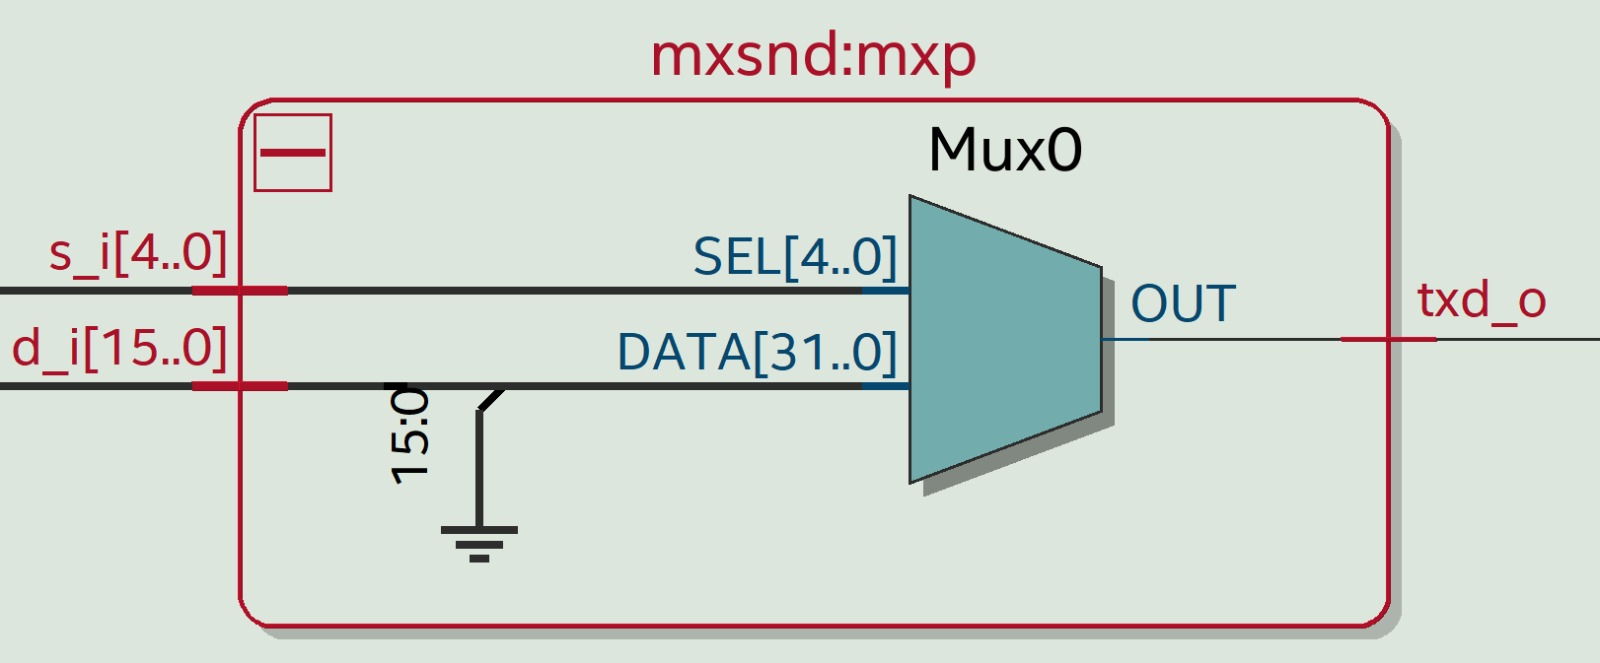
\includegraphics[scale=0.2]{../png/mxsnd_mxp.png}
	\caption{mxsnd\_mxp}
\end{figure}
\begin{center}
	\begin{tabular}{ | p{2cm} | c | c | p{5cm} |}
		\hline
		\textbf{Signal} & \textbf{Direction} & \textbf{Width} & \textbf{Description} \\
		\hline
		s\_i & IN & 5 & Bit position \\
		\hline
		d\_i & IN & 16 &  Bit vector \\
		\hline	
		txd\_o & OUT & 1 & txd, Serial Output \\
		\hline
	\end{tabular}
\end{center}

\newpage

\subsection{iffsm: FSM for Interface to S3}
This module contains the FSM for the 3-wire-interface to S3.
\begin{figure}[h]
	\centering	
	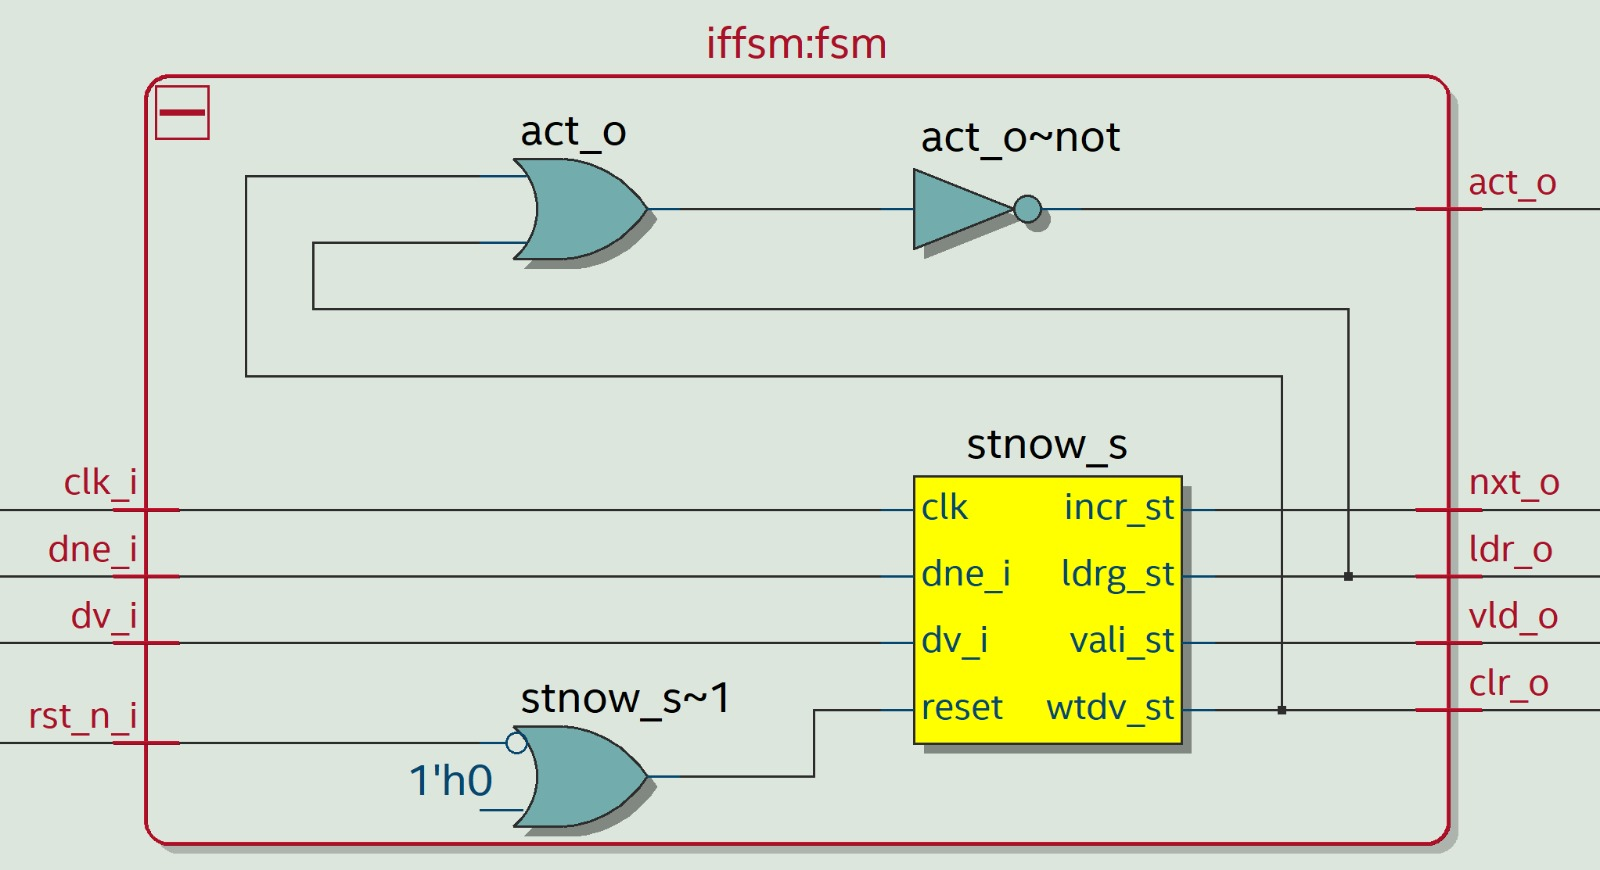
\includegraphics[scale=0.2]{../png/iffsm_fsm.png}
	\caption{iffsm\_fsm}
\end{figure}
\begin{center}
	\begin{tabular}{ | p{2cm} | c | c | p{5cm} |}
		\hline
		\textbf{Signal} & \textbf{Direction} & \textbf{Width} & \textbf{Description} \\
		\hline
		rst\_n\_i & IN & 1 & Reset, active low \\
		\hline
		clk\_i & IN & 1 & Syscp, @ 12MHz \\
		\hline
		dv\_i & IN & 1 & Have new RTC or GPS-Data \\
		\hline
		dne\_i & IN & 1 & Last Bit transmitted \\
		\hline
		ldr\_o & OUT & 1 & Enable register load \\
		\hline
		act\_o & OUT & 1 & Transmission active \\
		\hline
		vld\_o & OUT & 1 & Data Bit valid \\
		\hline
		clr\_o & OUT & 1 & Clear Bit-Counters \\
		\hline
		nxt\_o & OUT & 1 & Next Bit, inc count \\
		\hline
	\end{tabular}
\end{center}

\newpage

\subsection*{ifs3 - Finite State Machine}
\begin{figure}[h]
	\centering	
	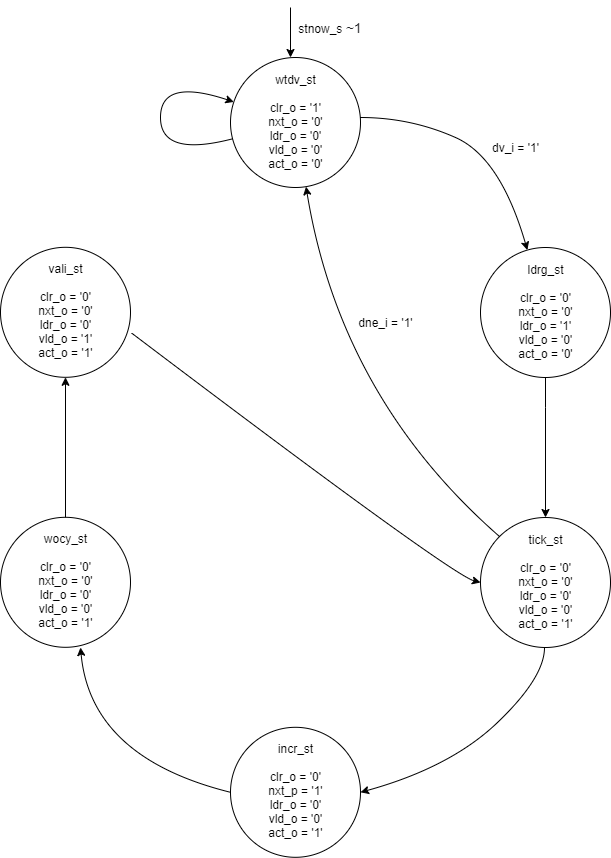
\includegraphics[scale=0.5]{../png/ifs3.png}
	\caption{ifs3 FSM}
\end{figure}
\begin{center}
 \begin{tabular}{| p{4cm} | p{7cm} |}
	 \hline
	 \textbf{State Name} & \textbf{Description} \\
	 \hline
	 wtdv\_st & wait until data valid \\
	 \hline
	 ldrg\_st & load data in register \\
	 \hline
	 tick\_st & check if done, else go on \\
	 \hline
	 incr\_st & get next bit (increment counter) \\
	 \hline
	 wocy\_st & wait one clock cycle \\
	 \hline
	 vali\_st & send validation bit \\
	 \hline
 \end{tabular}
\end{center}

\newpage

\chapter{Testbenches}
Testbenches are a great tool to test if the requirements are met. Our Project contains multiple testbenches to test the
important and complex modules. The trivial modules aren't tested directly, but they are tested in testbenches of modules 
with higher hiarchie aswell. \\ \\
\textbf{Testbenches:}
\begin{itemize}
	\item TB-top
	\item TB-clkgn
	\item TB-cntrl
	\item TB-dbpul
	\item TB-hdcnt
	\item TB-infs3
	\item TB-toggl
	\item TB-trigr
	\item TB-uatpc
\end{itemize}

\newpage

\chapter{Program Design}
The pc program is written in C++. It monitors a choosen COM-Port and receives the current number of people in the room when it changes.\\
The program is asking for a port number (between 0 and 10) and tries to open the serial connection afterwards. When an invalid number is entered, it tries to open the serial connection at the standard port COM5.
\begin{figure}[h]
	\centering	
	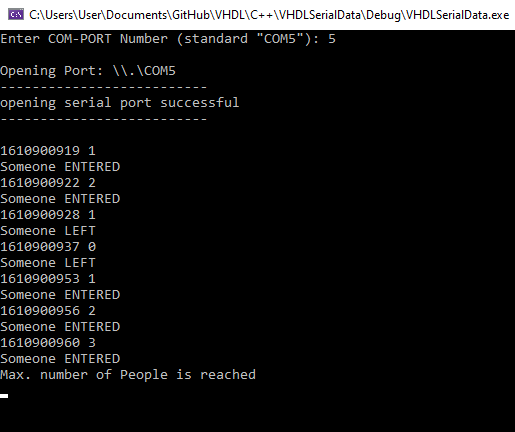
\includegraphics[scale=0.8]{../png/program.png}
	\caption{C++ Program Console}
\end{figure}
\begin{center}
	\begin{tabular}{|l|c|c|r|}
		\hline
		\textbf{Event} & \textbf{Beep One} & \textbf{Beep Two} & \textbf{Description} \\
		\hline
		Enter & LOW & HIGH & Someone entered the room \\
		\hline
		Leave & HIGH & LOW & Someone left the room \\
		\hline
		Stop & MEDIUM & MEDIUM & The room is full \\
		\hline
	\end{tabular}
\end{center}

\newpage

\chapter{Repository - Download}
The repository includes:
\begin{itemize}
	\item VHDL source code
	\item VHDL testbenches
	\item C++ source code
	\item Documentation/Specification
\end{itemize}
The lastest version of this project can be downloaded directly from \href{https://github.com/nlsy/VHDL}{https://github.com/nlsy/VHDL}. \\

\end{document}
